\documentclass[11pt,a4paper]{article}
\usepackage[utf8]{inputenc}
\usepackage[T1]{fontenc}
\usepackage{lmodern}
\usepackage[a4paper,margin=2.3cm]{geometry}
\usepackage{amsmath,amssymb,amsthm}
\usepackage{booktabs}
\usepackage{enumitem}
\usepackage{mathtools}
\usepackage{tikz}
\usetikzlibrary{positioning,arrows.meta,fit,backgrounds,calc,shapes.geometric,decorations.pathreplacing}
\usepackage{caption}
\usepackage[colorlinks=true,linkcolor=blue,citecolor=blue,urlcolor=blue]{hyperref}
\setlength{\parskip}{0.55em}
\setlength{\parindent}{0pt}

\newtheorem{theorem}{Theorem}[section]
\newtheorem{lemma}[theorem]{Lemma}
\newtheorem{definition}[theorem]{Definition}
\newtheorem{proposition}[theorem]{Proposition}
\newtheorem{corollary}[theorem]{Corollary}
\newtheorem{example}[theorem]{Example}
\newtheorem{remark}[theorem]{Remark}
\theoremstyle{remark}
\newtheorem*{intuition}{Intuition}
\newtheorem*{warning}{Warning}

\DeclareMathOperator{\rank}{rank}
\DeclareMathOperator{\diag}{diag}
\DeclareMathOperator{\spn}{span}
\DeclareMathOperator{\im}{im}
\DeclareMathOperator{\sgn}{sgn}
\DeclareMathOperator{\Ric}{Ric}
\DeclareMathOperator{\softmax}{softmax}
\DeclareMathOperator*{\argmax}{arg\,max}
\DeclareMathOperator*{\argmin}{arg\,min}
\DeclareMathOperator{\AUC}{AUC}
\DeclareMathOperator{\acc}{acc}
\DeclareMathOperator{\Spin}{Spin}

\newcommand{\Z}{\mathbb{Z}}
\newcommand{\R}{\mathbb{R}}
\newcommand{\C}{\mathbb{C}}
\newcommand{\N}{\mathbb{N}}
\newcommand{\E}{\mathbb{E}}
\newcommand{\Prob}{\mathbb{P}}
\newcommand{\Var}{\mathrm{Var}}
\newcommand{\Cov}{\mathrm{Cov}}
\newcommand{\GS}{G\"omb}
\newcommand{\sigmacycle}{$\sigma$-cycle}
\newcommand{\gp}{\otimes_{\mathrm{Cl}}}
\newcommand{\Cl}[2]{\mathrm{Cl}(#1, #2)}
\newcommand{\Quat}{\mathbb{H}}
\newcommand{\Tr}{\mathrm{Tr}}
\newcommand{\Id}{\mathrm{Id}}
\newcommand{\indic}[1]{\mathbf{1}\!\left[#1\right]}

\title{
  A long-form mathematical primer\\
  for HSiKAN, \GS{}-strict, \GS{}Soma, Sequential HSiKAN,\\
  and the $\sigma$-leakage audit framework
}
\author{Internal companion to the Nature Communications submission}
\date{2026-05-17}

\begin{document}
\maketitle

\begin{abstract}
This primer is a single-document refresher on every piece of
mathematics used by HSiKAN, \GS{}-strict (signed-graph link
prediction), \GS{}Soma (vision), Sequential HSiKAN $+$ CliffordFIR
(sequences), and the $\sigma$-leakage audit framework. It is
written to be read end-to-end in one or two evenings: the
definitions, the small number of theorems we actually rely on,
the proofs where they are short enough to clarify rather than
distract, and worked examples on the canonical datasets
(Bitcoin Alpha, Slashdot, Epinions, Cluttered MNIST).

Each section closes with a ``codebase'' pointer naming the file
that implements the construction so you can cross-reference math
and code without leaving the document.
\end{abstract}

\tableofcontents

\bigskip\bigskip
% ====================================================================
\part{Foundations of signed and hypergraph structure}
% ====================================================================

\section{Signed graphs, balance, and frustration}\label{sec:signed-graphs}

\subsection{Definitions}

\begin{definition}[Signed graph]
A \emph{signed graph} is a triple $G = (V, E, \sigma)$ where
\begin{itemize}[leftmargin=*]
\item $V$ is a finite vertex set with $|V| = n$;
\item $E \subseteq \binom{V}{2}$ is an undirected edge set (or
      $E \subseteq V \times V$ if directed) with $|E| = m$;
\item $\sigma : E \to \{-1, +1\}$ is a \emph{signature}.
\end{itemize}
The \emph{underlying graph} is $G^\pm = (V, E)$, obtained by
forgetting the signature. We write $E^+ = \sigma^{-1}(+1)$ and
$E^- = \sigma^{-1}(-1)$.
\end{definition}

\begin{definition}[Walk, path, cycle]
A \emph{walk} of length $k$ is an alternating sequence
$v_0, e_1, v_1, e_2, \dots, e_k, v_k$ with $e_i = (v_{i-1}, v_i)$;
a \emph{path} is a walk with all $v_i$ distinct; a \emph{cycle}
is a closed walk $v_0 = v_k$ with $v_0, v_1, \dots, v_{k-1}$
distinct.
\end{definition}

\begin{definition}[Cycle sign / $\sigma$-product]\label{def:cycle-sign}
For a cycle $c = (v_0, v_1, \dots, v_{k-1}, v_0)$ in a signed
graph $G$, the \emph{cycle sign} (or \emph{$\sigma$-product}) is
\[
  \sigma(c) \;\coloneqq\; \prod_{i=0}^{k-1} \sigma\bigl(v_i, v_{i+1 \bmod k}\bigr) \;\in\; \{-1, +1\}.
\]
\end{definition}

The cycle sign is the only signed invariant of a closed walk that
is permutation- and direction-invariant. In a signed graph,
\textbf{the structural data lives in the $\sigma$-products of
cycles}; anything not derivable from these is essentially an
unsigned-graph property.

\subsection{Switching equivalence}

\begin{definition}[Switching]
For a vertex subset $S \subseteq V$, the \emph{switch at $S$} of a
signed graph $G = (V, E, \sigma)$ is the new signed graph
$G^S = (V, E, \sigma^S)$ with
\[
  \sigma^S(e) \;=\;
  \begin{cases}
    -\sigma(e) & \text{if } e \text{ has exactly one endpoint in } S,\\
    +\sigma(e) & \text{otherwise.}
  \end{cases}
\]
Two signed graphs $G_1$ and $G_2$ on the same underlying graph are
\emph{switching-equivalent} if $G_2 = G_1^S$ for some
$S \subseteq V$.
\end{definition}

\begin{lemma}[Zaslavsky 1982]\label{lem:switching-invariant}
Switching preserves $\sigma$-cycle signs: if $G_2 = G_1^S$ then
for every cycle $c$, $\sigma_{G_1}(c) = \sigma_{G_2}(c)$.
\end{lemma}

\begin{proof}[Proof sketch]
Each edge with both endpoints in $S$ keeps its sign; each edge
with both endpoints outside $S$ keeps its sign; only edges with
exactly one endpoint in $S$ are negated. A cycle traversing the
boundary between $S$ and $V \setminus S$ crosses an even number
of such edges (each traversal in must be matched by a traversal
out), so the product of negations is $(-1)^{\text{even}} = +1$.
\end{proof}

\begin{intuition}
Switching is the signed-graph analogue of changing the sign
convention on a basis. If we negate the entire ``community A''
side of a network, every $\sigma$-product is unchanged: positive
edges between two community-A vertices stay positive (both
negated, $(-1)(-1) = +1$ on the path through them); but a single
crossing edge (one endpoint each in A and $\neg A$) gets negated.
\end{intuition}

\subsection{Balance theory}

\begin{figure}[h]
\centering
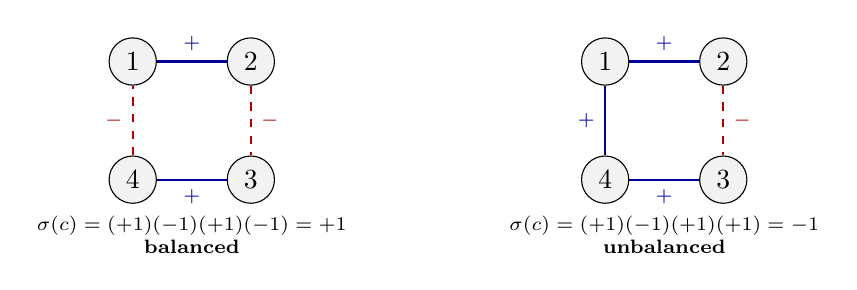
\begin{tikzpicture}[
  vertex/.style={circle, draw, fill=gray!10, minimum size=6mm, inner sep=0pt},
  posedge/.style={thick, blue!60!black},
  negedge/.style={thick, red!70!black, dashed},
  every label/.style={font=\scriptsize}
]
% Left graph: balanced (sigma(c) = +1)
\begin{scope}[xshift=-4cm]
\node[vertex] (a1) at (0, 1.5) {1};
\node[vertex] (a2) at (1.5, 1.5) {2};
\node[vertex] (a3) at (1.5, 0) {3};
\node[vertex] (a4) at (0, 0) {4};
\draw[posedge] (a1) -- node[above, font=\scriptsize]{$+$} (a2);
\draw[negedge] (a2) -- node[right, font=\scriptsize]{$-$} (a3);
\draw[posedge] (a3) -- node[below, font=\scriptsize]{$+$} (a4);
\draw[negedge] (a4) -- node[left, font=\scriptsize]{$-$} (a1);
\node[font=\scriptsize, align=center] at (0.75, -0.7)
  {$\sigma(c) = (+1)(-1)(+1)(-1) = +1$\\\textbf{balanced}};
\end{scope}
% Right graph: unbalanced (sigma(c) = -1)
\begin{scope}[xshift=2cm]
\node[vertex] (b1) at (0, 1.5) {1};
\node[vertex] (b2) at (1.5, 1.5) {2};
\node[vertex] (b3) at (1.5, 0) {3};
\node[vertex] (b4) at (0, 0) {4};
\draw[posedge] (b1) -- node[above, font=\scriptsize]{$+$} (b2);
\draw[negedge] (b2) -- node[right, font=\scriptsize]{$-$} (b3);
\draw[posedge] (b3) -- node[below, font=\scriptsize]{$+$} (b4);
\draw[posedge] (b4) -- node[left, font=\scriptsize]{$+$} (b1);
\node[font=\scriptsize, align=center] at (0.75, -0.7)
  {$\sigma(c) = (+1)(-1)(+1)(+1) = -1$\\\textbf{unbalanced}};
\end{scope}
\end{tikzpicture}
\caption{\textbf{Balanced vs unbalanced 4-cycles.} The
signature $\sigma : E \to \{-1, +1\}$ is the colour of each edge
(blue solid $=+1$, red dashed $=-1$). A cycle is balanced iff
its sign product is $+1$. The left graph has an even number of
negative edges; the right has an odd number.}
\label{fig:balanced-vs-unbalanced}
\end{figure}

\begin{definition}[Balanced graph]
A signed graph is \emph{balanced} if $\sigma(c) = +1$ for every
cycle $c \in G$.
\end{definition}

\begin{figure}[h]
\centering
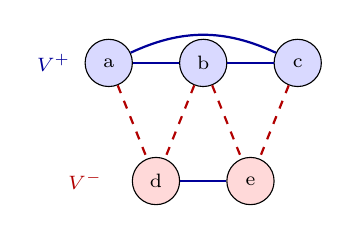
\begin{tikzpicture}[
  vertex/.style={circle, draw, fill=blue!15, minimum size=6mm, inner sep=0pt, font=\scriptsize},
  vertexB/.style={circle, draw, fill=red!15, minimum size=6mm, inner sep=0pt, font=\scriptsize},
  posedge/.style={thick, blue!60!black},
  negedge/.style={thick, red!70!black, dashed}
]
% Cartwright-Harary 2-partition example
\node[vertex] (a) at (0, 1) {a};
\node[vertex] (b) at (1.2, 1) {b};
\node[vertex] (c) at (2.4, 1) {c};
\node[vertexB] (d) at (0.6, -0.5) {d};
\node[vertexB] (e) at (1.8, -0.5) {e};
% within +
\draw[posedge] (a) -- (b);
\draw[posedge] (b) -- (c);
\draw[posedge] (a) to[bend left=25] (c);
\draw[posedge] (d) -- (e);
% across -
\draw[negedge] (a) -- (d);
\draw[negedge] (b) -- (d);
\draw[negedge] (b) -- (e);
\draw[negedge] (c) -- (e);
% Label the two partitions
\node[font=\scriptsize, blue!60!black] at (-0.7, 1) {$V^+$};
\node[font=\scriptsize, red!70!black] at (-0.3, -0.5) {$V^-$};
\end{tikzpicture}
\caption{\textbf{Cartwright--Harary 2-partition.} Theorem~\ref{thm:cartwright-harary}
guarantees that a balanced signed graph $G$ admits a partition
$V = V^+ \sqcup V^-$ such that within-partition edges are positive
(blue) and between-partition edges are negative (red dashed). The
two ``sides'' are the social communities; every closed walk that
crosses between them does so an even number of times, giving
$\sigma(c) = +1$.}
\label{fig:cartwright-harary}
\end{figure}

\begin{theorem}[Cartwright \& Harary 1956; Harary 1953]\label{thm:cartwright-harary}
The following are equivalent for a connected signed graph
$G = (V, E, \sigma)$:
\begin{enumerate}[label=(\roman*)]
\item Every cycle in $G$ has $\sigma(c) = +1$.
\item There exists a partition $V = V^+ \sqcup V^-$ such that all
      edges within $V^+$ and within $V^-$ are positive, and all
      edges between $V^+$ and $V^-$ are negative.
\item $G$ is switching-equivalent to the all-positive graph
      $(V, E, +1)$.
\end{enumerate}
\end{theorem}

\begin{proof}[Proof sketch]
$(i) \Rightarrow (ii)$: Pick a root vertex $v_0$ and put $v_0 \in
V^+$. For each other vertex $v$, choose a path $P$ from $v_0$ to
$v$ and put $v \in V^+$ if $\sigma(P) = +1$ and $v \in V^-$
otherwise. Independence of path choice: if $P, P'$ are two
$v_0$-to-$v$ paths, then $P \cup P^{\prime\,-1}$ is a closed walk
(possibly non-simple); by hypothesis its sign is $+1$, so
$\sigma(P) = \sigma(P')$, well-defining the partition. Verify the
sign condition on each edge directly.

$(ii) \Rightarrow (iii)$: Switch at $V^-$. Edges within $V^-$
stay positive (both endpoints negated, $(-)(-)=+$); cross edges
are negated $-1 \to +1$; within-$V^+$ edges are unchanged. Result
is all-positive.

$(iii) \Rightarrow (i)$: Lemma~\ref{lem:switching-invariant}:
switching preserves cycle signs; the all-positive graph has all
cycle signs $+1$; therefore $G$ does too.
\end{proof}

\subsection{Frustration}

Real-world networks are rarely balanced; we measure their
\emph{frustration} as a quantitative departure from balance.

\begin{definition}[Frustration index]
Given a signed graph $G$, the \emph{(edge) frustration index} is
\[
  L(G) \;=\; \min_{S \subseteq V}
              \bigl|\bigl\{ e \in E : \sigma^S(e) = -1 \bigr\}\bigr|,
\]
the minimum number of negative edges after any switching.
Equivalently, $L(G)$ is the minimum number of edges to delete
from $G$ to make it balanced.
\end{definition}

Computing $L(G)$ exactly is NP-hard (reduction from MAX-CUT), but
several proxies are tractable:
\begin{itemize}[leftmargin=*]
\item \emph{Cycle frustration:} the fraction of cycles in some
      reference pool $\mathcal{C}$ with $\sigma(c) = -1$. We compute
      this approximately by sampling cycles in
      \texttt{hymeko\_py/src/cycles/topk.rs}.
\item \emph{Triadic frustration:} the cycle-frustration measure
      restricted to triangles, computable in $O(m^{3/2})$ time
      via triangle listing.
\item \emph{Spectral frustration:} bounded by the smallest
      eigenvalue of the signed Laplacian (see \S\ref{sec:signed-laplacian}).
\end{itemize}

Empirical values on benchmark datasets:
\begin{center}
\begin{tabular}{lr@{\hspace{0.5em}}r}
\toprule
Dataset & $|V|$ & approx.\ triadic frustration \\
\midrule
Bitcoin Alpha & 3\,783 & $7\%$ \\
Bitcoin OTC   & 5\,881 & $9\%$ \\
Slashdot       & 82\,140 & $23\%$ \\
Epinions       & 131\,580 & $15\%$ \\
\bottomrule
\end{tabular}
\end{center}

\subsection{Spectral structure: the signed Laplacian}\label{sec:signed-laplacian}

\begin{definition}[Signed adjacency and Laplacian]
For a signed graph $G$, the \emph{signed adjacency matrix}
$A_\sigma \in \R^{n \times n}$ has entries $(A_\sigma)_{uv} =
\sigma(u, v)$ if $(u, v) \in E$, $0$ otherwise. The \emph{signed
degree} matrix $\bar D = \diag(\bar d)$ has $\bar d_u = \sum_v
|A_\sigma|_{uv}$ (the unsigned degree). The \emph{signed
Laplacian} is
\[
  L_\sigma \;=\; \bar D - A_\sigma.
\]
\end{definition}

Note the use of unsigned degrees in $\bar D$: this makes
$L_\sigma$ \emph{positive semidefinite} (unlike the naive
$D - A_\sigma$ with signed degrees, which can have negative
eigenvalues for unbalanced graphs).

\begin{proposition}[Kunegis et al.\ 2010]\label{prop:laplacian-balance}
For a connected signed graph $G$, the smallest eigenvalue
$\lambda_1(L_\sigma) = 0$ if and only if $G$ is balanced.
Otherwise $\lambda_1(L_\sigma) > 0$, and the gap quantifies
distance-to-balance.
\end{proposition}

\begin{proof}[Proof sketch]
$\lambda_1 \geq 0$ by Gershgorin (every row of $L_\sigma$ has
diagonal $\bar d_u$ and off-diagonal absolute-sum $\bar d_u$).
For the iff: $\lambda_1 = 0$ with eigenvector $f$ means
$\bar d_u f_u = \sum_v A_\sigma(u,v) f_v$ for every $u$; rearranging,
$\sigma(u,v) f_u f_v = f_v^2$ (after multiplying both sides by
$f_v$ and re-summing), which on a connected graph forces $|f_u| =
|f_v|$ for all $u, v$ and $\sigma(u, v) = \sgn(f_u f_v)$. This is
exactly the balance partition.
\end{proof}

\subsection{Codebase pointers}

\begin{tabular}{ll}
Signed-graph data class & \texttt{signedkan\_wip/src/datasets.py:SignedGraph} \\
Bitcoin / Slashdot / Epinions loader & \texttt{signedkan\_wip/src/datasets.py:load} \\
Reddit Hyperlinks loader (Phase C) & \texttt{datasets.py:load("reddit\_body" / "reddit\_title")} \\
\end{tabular}

% ====================================================================
\section{Cycles: enumeration, scoring, and pooling}\label{sec:cycles}

\subsection{Cycle enumeration is hard}

Listing all cycles of length exactly $k$ in a graph is
$\#$P-hard in general; even just counting $4$-cycles is
intractable for dense graphs. The standard tractable strategies
are:

\begin{enumerate}[label=(\Roman*)]
\item \emph{Full enumeration with hard cap} for small graphs and
      small $k$. Bitcoin Alpha at $k = 5$: 171\,358 cycles, fits
      in memory. Slashdot at $k = 5$: $> 55$ million, doesn't.
\item \emph{Color-coding} (Alon, Yuster, Zwick 1995): random
      $k$-coloring of $V$; cycles are enumerated only if
      \emph{colourful} (all vertices distinct colors). Repeat
      $O(\binom{k}{k/2})$ times for a constant-factor approximation.
\item \emph{Branch-and-bound by per-vertex score} with a sum-of-
      sub-path-bounds upper-bound function (see
      \S\ref{ssec:branch-and-bound}).
\item \emph{Walk closure}: enumerate length-$(k-1)$ walks, check
      if the missing edge closes the walk into a cycle.
\end{enumerate}

\subsection{Branch-and-bound enumeration with bounded scores}\label{ssec:branch-and-bound}

For top-$m$-per-vertex cycle selection with score function
$s : \mathcal{C} \to \R_{\geq 0}$, we maintain a per-vertex heap
of size $m$ during DFS. The DFS explores a tree of partial paths
$P = (v_0, v_1, \dots, v_\ell)$ with $\ell < k$. We need an
\emph{upper bound} on the maximum score of any cycle extending
$P$.

\begin{definition}[Bounded scorer]
A score function $s$ is \emph{bounded} if there exists
$\bar s : (\text{partial path}) \to \R_{\geq 0}$ such that for every
partial path $P$ and every cycle $c$ extending $P$,
\[
  s(c) \;\leq\; \bar s(P).
\]
\end{definition}

If the heap is already full of cycles of score $\geq s^\star$,
we can prune the DFS branch at $P$ whenever $\bar s(P) \leq s^\star$.
This is the core speedup behind the ABB enumerator
(\texttt{hymeko\_py/src/cycles/topk.rs}): on Epinions at $k = 5$,
ABB takes $4.0$ s for $K = 10$k cycles versus $100.5$ s for the
non-bounded enumerator.

\subsection{Scoring functions}

\begin{description}[font=\normalfont\emph]
\item[Balance fraction] $s_{\text{bal}}(c) = \indic{\sigma(c) = +1}$.
      Counts balanced cycles. Bounded: a partial path either
      already contains a $\sigma = -1$ edge (so the final cycle
      sign is at best $-1$) or doesn't (final at best $+1$).
\item[Davis index] $s_{\text{Dav}}(c) = \indic{c \text{ has all-positive or all-negative or mixed-balanced pattern}}$.
      Generalises balance to triadic patterns.
\item[Unbalanced fraction] $s_{\text{unbal}}(c) = \indic{\sigma(c) = -1}$.
      Counts unbalanced cycles --- the dual of $s_{\text{bal}}$.
\item[Weighted sum] $s_{\text{w}}(c) = \sum_i w_i \cdot \text{feature}_i(c)$
      for arbitrary feature combinations.
\end{description}

The \emph{ABB} extension of these scorers tracks both an upper
and lower bound on the cycle score as the DFS extends, allowing
branch pruning when the upper bound falls below the heap floor.

\subsection{$\sigma$-cycle pooling}

\begin{definition}[Cycle pool of arity $k$]
$\mathcal{C}_k(G) \;\coloneqq\; \{c : c \text{ is a $k$-cycle in } G\}$,
with each cycle counted once up to rotation and reflection.
\end{definition}

\begin{definition}[$\sigma$-weighted cycle pool feature]
Given per-vertex embeddings $h_v \in \R^d$ and a cycle
$c = (v_0, \dots, v_{k-1}, v_0)$, define a per-cycle feature
$\phi(c) = \mathrm{Aggregate}(h_{v_0}, \dots, h_{v_{k-1}})$ via
some permutation-invariant aggregator (mean, max, sum). The
\emph{$\sigma$-weighted cycle pool feature} for vertex $v$ is
\[
  z_v^{(k)} \;\coloneqq\; \sum_{c \in \mathcal{C}_k(G) : v \in c}
                            \sigma(c) \cdot \phi(c).
\]
\end{definition}

\paragraph{Why $\sigma$-weighting matters.}
Without the $\sigma(c)$ factor, $z_v^{(k)}$ depends only on the
underlying graph and the per-vertex embeddings --- the signature
$\sigma$ is forgotten. The $\sigma$-weighted variant is the
simplest aggregator that uses cycle-level signed structure.

\subsection{Mixed-arity pooling and the $\alpha_k$ simplex}

For $k \in \mathcal{K} \subseteq \{3, 4, 5, 6\}$, we compute
$z_v^{(k)}$ for each arity, then mix:
\[
  z_v \;=\; \sum_{k \in \mathcal{K}} \alpha_k \, z_v^{(k)},
  \qquad \alpha = \softmax(\theta).
\]
$\theta$ is learned jointly with the rest of the network. The
learned distribution $\alpha$ acts as a \emph{regime compass}:

\begin{center}
\begin{tabular}{lcccc}
\toprule
Dataset & $\alpha_3$ & $\alpha_4$ & $\alpha_5$ & dominant \\
\midrule
Bitcoin Alpha & $\sim 0.04$ & $\sim 0.45$ & $\sim 0.51$ & $4 + 5$ \\
Bitcoin OTC   & $\sim 0.06$ & $\sim 0.49$ & $\sim 0.45$ & $4 + 5$ \\
Slashdot      & $\sim 0.18$ & $\sim 0.36$ & $\sim 0.46$ & $5$ \\
Epinions      & $\sim 0.22$ & $\sim 0.39$ & $\sim 0.39$ & $4 + 5$ \\
SBM $k = 4$ (synthetic) & $\sim 0.55$ & $\sim 0.40$ & $\sim 0.05$ & $3$ \\
\bottomrule
\end{tabular}
\end{center}

\subsection{Walk-vs-cycle: when walks add value}

A cycle of length $k$ contains $\binom{k}{2}$ shorter walks. A
\emph{walk-only aggregator} (used in the Walk-HSiKAN variant) sums
over open walks instead of closed cycles, with the walk's product
of edge signs replacing the cycle's $\sigma$. Walks help in two
regimes:

\begin{enumerate}
\item Very sparse graphs where cycles are rare. SBM $k = 4$ at
      $|V| = 200$ has only $\sim 5$k $4$-cycles but $\sim 30$k
      length-$4$ walks.
\item Heterogeneous-degree graphs where high-degree hub vertices
      participate in many walks not closed into cycles. Slashdot
      and Epinions both show this regime.
\end{enumerate}

\subsection{Codebase pointers}

\begin{tabular}{ll}
DFS cycle enumeration (Rust) & \texttt{hymeko\_py/src/cycles/dfs.rs} \\
Color-coded enumeration & \texttt{hymeko\_py/src/cycles/color\_coded.rs} \\
Path-closure heuristic & \texttt{hymeko\_py/src/cycles/path\_closure.rs} \\
Top-$m$ ABB enumerator & \texttt{hymeko\_py/src/cycles/topk.rs} \\
Cycle scorers & \texttt{hymeko\_py/src/cycles/scorers.rs} \\
Cycle pool aggregator (Python) & \texttt{signedkan\_wip/src/n\_tuples.py} \\
\end{tabular}

\bigskip
% ====================================================================
\part{Function approximation: KAN and HSiKAN}
% ====================================================================

\section{The Kolmogorov-Arnold representation}\label{sec:ka}

\subsection{The classical theorem}

\begin{theorem}[Kolmogorov 1957]\label{thm:kolmogorov}
For every continuous $f : [0, 1]^n \to \R$ there exist continuous
univariate functions
$\Phi_0, \Phi_1, \dots, \Phi_{2n} : \R \to \R$ and
$\varphi_{q, p} : \R \to \R$ for $q \in \{0, \dots, 2n\}$ and
$p \in \{1, \dots, n\}$ such that
\[
  f(x_1, \dots, x_n) \;=\; \sum_{q = 0}^{2n} \Phi_q\!\left( \sum_{p = 1}^{n} \varphi_{q, p}(x_p) \right).
\]
\end{theorem}

The Sprecher refinement (Sprecher 1965) shows that the inner
$\varphi_{q, p}$ can be chosen \emph{universal} (independent of $f$),
so the outer $\Phi_q$ alone carry the function-specific information.

\paragraph{What the theorem says, plainly.} Every continuous
multivariate function decomposes into a stack of two univariate
transformations summed at one intermediate layer of width $2n + 1$.
This is the original ``deep learning'' theorem, predating MLPs by
two decades.

\paragraph{What the theorem does \emph{not} say.} It does not say
the inner functions are smooth. In Kolmogorov's original
construction the $\varphi_{q, p}$ are Lipschitz but not $C^1$;
in fact they cannot be smooth, as a celebrated result of Vitushkin
(1954) shows that smooth Kolmogorov representations don't exist
for generic $f$. This non-smoothness is exactly why naive
``per-edge learnable activation'' networks are notoriously
unstable to train.

\subsection{From the theorem to the KAN architecture}

The KAN (Kolmogorov-Arnold Network) architecture of Liu et al.\
(2024) approximates a Kolmogorov representation by parameterising
each $\varphi$ and $\Phi$ as a smooth basis-function expansion. A
single ``KAN layer'' replaces the MLP's
$\mathbf{y} = \sigma(W \mathbf{x} + b)$ with
\[
  y_j \;=\; \sum_{i} \varphi_{j, i}(x_i),
\]
where each $\varphi_{j, i}$ is its own learnable univariate
function. Stacking $L$ such layers gives the full KAN.

\subsection{Univariate basis: B-splines vs Catmull-Rom}

\begin{definition}[Cubic B-spline basis]
For knots $t_0 < t_1 < \dots < t_{G-1}$, the cubic B-spline basis
functions $B_i^{(3)} : \R \to \R$ are recursively defined by
\[
  B_i^{(0)}(x) \;=\; \indic{t_i \leq x < t_{i+1}},
  \qquad
  B_i^{(k)}(x) \;=\; \frac{x - t_i}{t_{i+k} - t_i} B_i^{(k-1)}(x)
                     + \frac{t_{i+k+1} - x}{t_{i+k+1} - t_{i+1}} B_{i+1}^{(k-1)}(x).
\]
A function $\varphi : \R \to \R$ is represented as
$\varphi(x) = \sum_i c_i B_i^{(3)}(x)$ with learnable coefficients
$c_i$.
\end{definition}

B-splines have global support (each $B_i$ is non-zero over the
interval $[t_i, t_{i+4}]$). For learning, this means a single
function evaluation touches all 4 neighbouring control points,
which is fine, but the basis is not interpolating: the function
does \emph{not} pass through any specific control values.

\begin{definition}[Catmull-Rom spline]
For knots $t_0 < t_1 < \dots < t_{G-1}$ and control values
$y_0, y_1, \dots, y_{G-1}$, the cubic Catmull-Rom interpolant
on the interval $[t_i, t_{i+1}]$ is, with $t = (x - t_i)/(t_{i+1} - t_i)$,
\[
  \varphi(x) \;=\; \frac{1}{2}
  \begin{pmatrix} 1 & t & t^2 & t^3 \end{pmatrix}
  \begin{pmatrix}
    0 & 2 & 0 & 0 \\
    -1 & 0 & 1 & 0 \\
    2 & -5 & 4 & -1 \\
    -1 & 3 & -3 & 1
  \end{pmatrix}
  \begin{pmatrix} y_{i-1} \\ y_i \\ y_{i+1} \\ y_{i+2} \end{pmatrix}.
\]
\end{definition}

\begin{proposition}[Catmull-Rom properties]
The Catmull-Rom interpolant on each interval is cubic in $t$,
$C^1$-continuous across knot boundaries, and \emph{interpolates}
the control values: $\varphi(t_i) = y_i$ for all $i$.
\end{proposition}

We use Catmull-Rom (rather than B-splines) for the HSiKAN
activations because the interpolation property gives a clean
identity initialisation: setting $y_i = t_i$ makes the function
the identity, recovering the linear-no-nonlinearity baseline at
init. (B-spline initialisation requires solving a least-squares
problem to invert the basis.)

\paragraph{Computational cost.} Each Catmull-Rom evaluation is
$O(1)$: identify the interval (binary search over $G$ knots,
$O(\log G)$ in general but $O(1)$ for fixed-grid Catmull-Rom),
multiply the $4 \times 4$ matrix times the control vector. For
$d_{\text{channels}} = 32$ and $G = 8$ knots, each layer is
$32 \times 8 = 256$ scalar parameters versus an MLP's $32 \times 32 =
1024$ --- the KAN layer is $4 \times$ parameter-cheaper at this
configuration.

\subsection{The HSiKAN aggregator}\label{ssec:hsikan-aggregator}

\begin{definition}[HSiKAN $\sigma$-masked aggregator]
Given per-vertex features $\{h_i\}_{i = 1}^k$ at the corners of a
$k$-cycle with signs $\{\sigma_i\}_{i=1}^k \in \{-1, +1\}^k$, the
HSiKAN aggregator computes:
\begin{align*}
  u_{i, +} &= \varphi_{\text{in}}^{(+)}(h_i)                                 && (\text{per-corner, pos branch}) \\
  u_{i, -} &= \varphi_{\text{in}}^{(-)}(h_i)                                 && (\text{per-corner, neg branch}) \\
  a_+      &= \frac{1}{|\{i : \sigma_i = +1\}|}
              \sum_{i : \sigma_i = +1} u_{i, +}                                  && (\text{pos pool}) \\
  a_-      &= \frac{1}{|\{i : \sigma_i = -1\}|}
              \sum_{i : \sigma_i = -1} u_{i, -}                                  && (\text{neg pool}) \\
  z        &= \varphi_{\text{out}}^{(+)}(a_+) \;+\; \varphi_{\text{out}}^{(-)}(a_-) && (\text{output stack})
\end{align*}
where each $\varphi : \R^d \to \R^d$ is a per-channel Catmull-Rom
activation (4 in total: in+, in--, out+, out--).
\end{definition}

\begin{figure}[h]
\centering
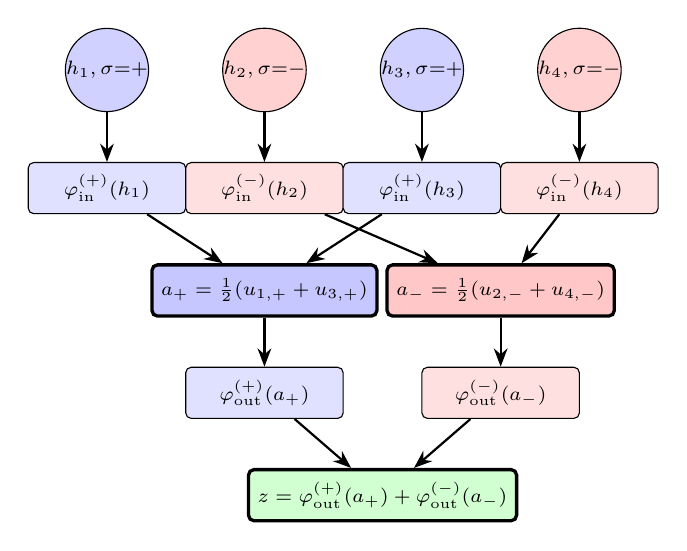
\begin{tikzpicture}[
  every node/.style={font=\scriptsize},
  corner/.style={circle, draw, fill=gray!10, minimum size=6mm, inner sep=0pt},
  cornerP/.style={circle, draw, fill=blue!18, minimum size=6mm, inner sep=0pt},
  cornerN/.style={circle, draw, fill=red!18, minimum size=6mm, inner sep=0pt},
  block/.style={draw, rounded corners=2pt, minimum width=2.0cm, minimum height=0.65cm, align=center},
  pblock/.style={block, fill=blue!12},
  nblock/.style={block, fill=red!12},
  poolP/.style={block, fill=blue!22, very thick},
  poolN/.style={block, fill=red!22, very thick},
  outblock/.style={block, fill=green!18, very thick},
  flow/.style={->, thick, >=Stealth}
]
% Input corners with signs
\node[cornerP] (h1) at (0, 4) {$h_1, \sigma{=}+$};
\node[cornerN] (h2) at (2, 4) {$h_2, \sigma{=}-$};
\node[cornerP] (h3) at (4, 4) {$h_3, \sigma{=}+$};
\node[cornerN] (h4) at (6, 4) {$h_4, \sigma{=}-$};
% Per-sign branches
\node[pblock] (u1p) at (0, 2.5) {$\varphi_\text{in}^{(+)}(h_1)$};
\node[nblock] (u2n) at (2, 2.5) {$\varphi_\text{in}^{(-)}(h_2)$};
\node[pblock] (u3p) at (4, 2.5) {$\varphi_\text{in}^{(+)}(h_3)$};
\node[nblock] (u4n) at (6, 2.5) {$\varphi_\text{in}^{(-)}(h_4)$};
\draw[flow] (h1) -- (u1p);
\draw[flow] (h2) -- (u2n);
\draw[flow] (h3) -- (u3p);
\draw[flow] (h4) -- (u4n);
% Pools
\node[poolP] (poolp) at (2, 1.2) {$a_+ = \frac{1}{2}(u_{1,+} + u_{3,+})$};
\node[poolN] (pooln) at (5, 1.2) {$a_- = \frac{1}{2}(u_{2,-} + u_{4,-})$};
\draw[flow] (u1p) -- (poolp);
\draw[flow] (u3p) -- (poolp);
\draw[flow] (u2n) -- (pooln);
\draw[flow] (u4n) -- (pooln);
% Per-sign output
\node[pblock] (outp) at (2, -0.1) {$\varphi_\text{out}^{(+)}(a_+)$};
\node[nblock] (outn) at (5, -0.1) {$\varphi_\text{out}^{(-)}(a_-)$};
\draw[flow] (poolp) -- (outp);
\draw[flow] (pooln) -- (outn);
% Sum
\node[outblock] (z) at (3.5, -1.4) {$z = \varphi_\text{out}^{(+)}(a_+) + \varphi_\text{out}^{(-)}(a_-)$};
\draw[flow] (outp) -- (z);
\draw[flow] (outn) -- (z);
\end{tikzpicture}
\caption{\textbf{The HSiKAN $\sigma$-masked aggregator.} A
4-cycle with two positive and two negative edges. Per-corner
features pass through sign-specific Catmull--Rom activations
$\varphi_\text{in}^{(\pm)}$, the per-sign pools $a_\pm$ average
the corners of each sign, and the output stacks
$\varphi_\text{out}^{(\pm)}$ produce the final aggregator output.
The architecture is permutation-invariant within each sign
class.}
\label{fig:hsikan-aggregator}
\end{figure}

\begin{figure}[h]
\centering
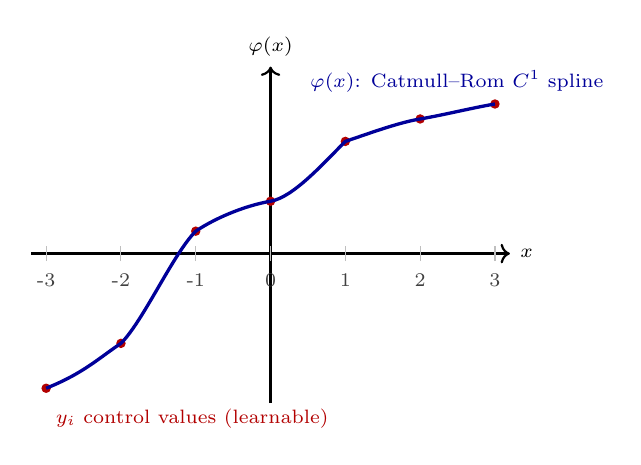
\begin{tikzpicture}[scale=0.95]
% Plot region
\def\xmin{-3.2}
\def\xmax{3.2}
\def\ymin{-2.0}
\def\ymax{2.5}
% Axes
\draw[->, thick] (\xmin, 0) -- (\xmax, 0) node[right, font=\scriptsize] {$x$};
\draw[->, thick] (0, \ymin) -- (0, \ymax) node[above, font=\scriptsize] {$\varphi(x)$};
% Control points (knots): place at x = -3, -2, -1, 0, 1, 2, 3 with various y values
\foreach \px/\py in {-3/-1.8, -2/-1.2, -1/0.3, 0/0.7, 1/1.5, 2/1.8, 3/2.0} {
  \fill[red!70!black] (\px, \py) circle (1.8pt);
}
% Approximate the Catmull-Rom-like interpolant as a smooth path through the points.
% Use a hand-crafted curved path that passes through each.
\draw[blue!60!black, very thick, smooth]
  (-3, -1.8) .. controls (-2.5, -1.6) and (-2.3, -1.4) ..
  (-2, -1.2) .. controls (-1.7, -0.9) and (-1.3, -0.0) ..
  (-1, 0.3)  .. controls (-0.7, 0.5) and (-0.3, 0.65) ..
  ( 0, 0.7)  .. controls ( 0.3, 0.75) and ( 0.7, 1.2) ..
  ( 1, 1.5)  .. controls ( 1.3, 1.6) and ( 1.7, 1.75) ..
  ( 2, 1.8)  .. controls ( 2.3, 1.85) and ( 2.7, 1.95) ..
  ( 3, 2.0);
% Labels
\node[font=\scriptsize, red!70!black, anchor=west] at (-3.0, -2.2) {$y_i$ control values (learnable)};
\node[font=\scriptsize, blue!60!black, anchor=west] at ( 0.4, 2.3) {$\varphi(x)$: Catmull--Rom $C^1$ spline};
% knot ticks
\foreach \px in {-3, -2, -1, 0, 1, 2, 3} {
  \draw[gray!50] (\px, -0.1) -- (\px, 0.1);
  \node[font=\scriptsize, gray!50!black] at (\px, -0.35) {\px};
}
\end{tikzpicture}
\caption{\textbf{Catmull--Rom spline activation.} The learnable
univariate function $\varphi : \R \to \R$ is a $C^1$ cubic
interpolant through learnable control values $y_i$ at fixed knot
positions $x_i$. Inputs outside $[x_0, x_{G-1}]$ extrapolate
linearly using the boundary slopes (clamped); inside the range
the spline is exact at each knot. Setting $y_i = x_i$ initialises
$\varphi$ to the identity (no nonlinearity at init).}
\label{fig:catmull-rom}
\end{figure}

\subsubsection{Expressiveness}

\begin{proposition}[HSiKAN universal approximation]
The HSiKAN aggregator with sufficiently many knots per channel
is a universal approximator for continuous permutation-invariant
functions $f : (\R^d)^k \times \{-1, +1\}^k \to \R^d$.
\end{proposition}

\begin{proof}[Proof sketch]
By Theorem~\ref{thm:kolmogorov}, any continuous $f$ admits a
Kolmogorov representation. The $\sigma$-masked pooling exactly
implements the inner-sum step (with separate sums for the two
sign classes); the per-channel Catmull-Rom approximation of
$\varphi_{\text{in/out}}$ is dense in continuous univariates as
the knot count grows.
\end{proof}

\subsubsection{Why $\sigma$-masking changes the function class}

Suppose we drop the $\sigma$-mask and just pool all $k$ corners
together: $a = \frac{1}{k} \sum_i \varphi_{\text{in}}(h_i)$. Then
$a$ is invariant to a sign flip of \emph{any} subset of
$\{\sigma_i\}$, so the aggregator gets no information about the
signature. The $\sigma$-masked pool, by contrast, splits the
signal: $a_+$ tracks the positive-edge corners' features,
$a_-$ tracks the negative; the output stack combines them in a
sign-aware way.

\paragraph{The $\sigma$-product interpretation.} The HSiKAN aggregator
applied to a cycle is, after one layer, mathematically equivalent
to a sign-aware mixture model with the partition implied by
$\{\sigma_i\}_{i=1}^k$. Iterated over cycle layers (the cascade
in \GS{}-strict), the global function evaluates a polynomial in
the cycle $\sigma$-products of bounded degree.

\subsection{Codebase pointers}

\begin{tabular}{ll}
Catmull-Rom activation (vision) & \texttt{signedkan\_wip/src/vision/hymeyolo\_backbones.py:CatmullRomActivation} \\
HSiKAN aggregator (vision) & \texttt{signedkan\_wip/src/vision/hymeyolo\_q\_smoke.py:HSiKANAggregator} \\
Mixed-arity SignedKAN config & \texttt{signedkan\_wip/src/mixed\_arity\_signedkan/} \\
$\alpha_k$ softmax mixer & \texttt{signedkan\_wip/src/mixed\_arity\_signedkan/model.py:alpha\_logits} \\
\end{tabular}

\bigskip
% ====================================================================
\part{Hypergraph cycle pooling: the G\"omb cascade}
% ====================================================================

\section{Signed hypergraphs}\label{sec:signed-hyper}

\subsection{Definitions}

\begin{definition}[Signed hypergraph]
A \emph{signed hypergraph} is a triple $H = (V, \mathcal{E}, \sigma)$
where $\mathcal{E} \subseteq 2^V$ is a collection of hyperedges
(each $e \in \mathcal{E}$ is a subset of $V$ with $|e| \geq 2$),
and $\sigma : \mathcal{E} \to \{-1, +1\}$.
\end{definition}

\begin{definition}[Signed incidence matrix]
For a signed hypergraph $H = (V, \mathcal{E}, \sigma)$, the
\emph{signed incidence matrix} $M_\sigma \in \R^{|V| \times |\mathcal{E}|}$
has entries
\[
  (M_\sigma)_{v, e} \;=\;
  \begin{cases}
    \sigma(e) & \text{if } v \in e, \\
    0 & \text{otherwise.}
  \end{cases}
\]
\end{definition}

For graphs $(|e| = 2)$ this is the standard sign-weighted
edge-vertex incidence matrix. The columns are sign-tagged
indicator vectors of the hyperedges' vertex sets.

\subsection{Cycle-as-hyperedge}

The bridge from a signed graph to a hypergraph: for each cycle
$c$ in the underlying $G$, treat the vertex set
$\{v_0, \dots, v_{k-1}\}$ as a single hyperedge of arity $k$,
carrying the sign $\sigma(c)$. The resulting hypergraph has
$|\mathcal{E}_c| = |\mathcal{C}_k(G)|$ hyperedges, all of cardinality
$k$, with sign equal to the cycle $\sigma$-product.

This construction is what \GS{}-strict's middle shell consumes.
The signed incidence matrix at this layer carries the cycle-level
structural data; the cascade lifts it through three nested
operators (see \S\ref{sec:gomb-cascade}).

\subsection{Hypergraph Laplacians}

\begin{definition}[Unsigned hypergraph Laplacian, Chung 1997]
For an unsigned hypergraph $H = (V, \mathcal{E})$ with incidence
$M$ (each entry $\indic{v \in e}$), the standard hypergraph
Laplacian is
\[
  L_H \;=\; D_V - M \, D_E^{-1} M^\top,
\]
where $D_V \in \R^{|V| \times |V|}$ is the diagonal of vertex
degrees $d(v) = |\{e : v \in e\}|$ and $D_E \in
\R^{|\mathcal{E}| \times |\mathcal{E}|}$ is the diagonal of
hyperedge sizes $|e|$.
\end{definition}

For signed hypergraphs we use $M_\sigma$ in place of $M$ (with
unsigned degrees in $D_V$). The construction generalises the
signed-graph Laplacian of \S\ref{sec:signed-laplacian}: the
balance theorem extends, with the smallest eigenvalue of the
signed hypergraph Laplacian being zero iff the cycle-as-hyperedge
construction is balanced.

\subsection{Codebase pointers}

\begin{tabular}{ll}
Signed incidence (Python) & \texttt{signedkan\_wip/src/hymeko\_gomb/cascade.py} \\
Hypergraph convolution & \texttt{signedkan\_wip/src/hymeko\_gomb/soma/hg\_conv\_bochner.py} \\
\end{tabular}

\section{The G\"omb three-shell cascade}\label{sec:gomb-cascade}

\begin{figure}[h]
\centering
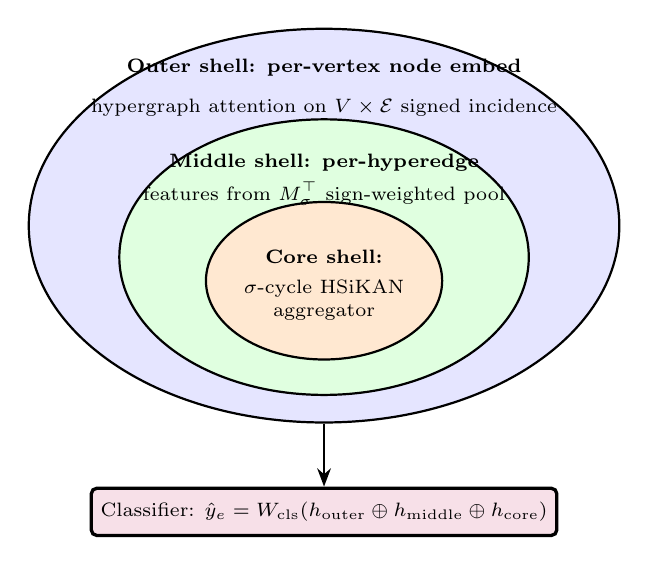
\begin{tikzpicture}[
  every node/.style={font=\scriptsize},
  outer/.style={ellipse, draw, fill=blue!10, minimum width=7.5cm, minimum height=5.0cm, thick},
  middle/.style={ellipse, draw, fill=green!12, minimum width=5.2cm, minimum height=3.5cm, thick},
  core/.style={ellipse, draw, fill=orange!18, minimum width=3.0cm, minimum height=2.0cm, thick},
  cls/.style={draw, rounded corners=2pt, fill=purple!12, minimum width=3.0cm, minimum height=0.6cm, very thick}
]
\node[outer] (outer) at (0, 0) {};
\node[middle] (middle) at (0, -0.4) {};
\node[core] (core) at (0, -0.7) {};
\node[font=\scriptsize\bfseries] at (0, 2.0) {Outer shell: per-vertex node embed};
\node[font=\scriptsize] at (0, 1.5) {hypergraph attention on $V \times \mathcal{E}$ signed incidence};
\node[font=\scriptsize\bfseries] at (0, 0.8) {Middle shell: per-hyperedge};
\node[font=\scriptsize] at (0, 0.4) {features from $M_\sigma^\top$ sign-weighted pool};
\node[font=\scriptsize\bfseries] at (0, -0.4) {Core shell:};
\node[font=\scriptsize] at (0, -0.8) {$\sigma$-cycle HSiKAN};
\node[font=\scriptsize] at (0, -1.1) {aggregator};
% Output to classifier
\node[cls, below=0.8 of outer] (cls) {Classifier:  $\hat y_e = W_\text{cls}(h_\text{outer} \oplus h_\text{middle} \oplus h_\text{core})$};
\draw[->, thick, >=Stealth] (outer.south) -- (cls.north);
\end{tikzpicture}
\caption{\textbf{The \GS{}-strict three-shell cascade.} Three
nested shells operate at successively richer signed-structure
levels: outer (per-vertex), middle (per-hyperedge), core (per-
cycle $\sigma$-product). The final classifier consumes a
concatenation of all three.}
\label{fig:gomb-cascade}
\end{figure}

\subsection{Architecture overview}

\GS{}-strict processes a signed graph through three nested
``shells'', each operating at a different abstraction level:

\begin{enumerate}[label=\textbf{Shell \arabic*:}, leftmargin=2.2cm]
\item \emph{Outer.} Per-vertex node embeddings via a hypergraph
      attention pass. Dimension $d_{\text{outer}}$. Operates on
      the original $|V| \times |\mathcal{E}|$ signed-incidence
      tensor.
\item \emph{Middle.} Per-hyperedge features computed from the
      outer-shell node embeddings projected through $M_\sigma^\top$
      (the transpose carries per-edge sign-weighted vertex pool).
      Dimension $d_{\text{middle}}$.
\item \emph{Core.} Cycle pool aggregator from
      \S\ref{sec:cycles}, with the HSiKAN factorisation from
      \S\ref{ssec:hsikan-aggregator}. Dimension $d_{\text{core}}$.
\end{enumerate}

The final classifier takes a sum of all three shells'
contributions:
\[
  \hat y_e \;=\; W_{\text{cls}}\!\left( h_{\text{outer}, e}
                     \oplus h_{\text{middle}, e}
                     \oplus h_{\text{core}, e} \right),
\]
where $\oplus$ is concatenation and $h_{\text{shell}, e}$ is the
per-edge feature derived from each shell.

\subsection{Tier organisation: hierarchical $n_{\text{tiers}}$}

\GS{}-strict supports an \emph{intrastructural tier} dimension
$n_{\text{tiers}}$. Each shell is replicated $n_{\text{tiers}}$
times with shared per-tier weights but distinct routing, allowing
the model to specialise different tiers to different cycle
sub-pools. This is configurable per shell (e.g.\ Bitcoin Alpha's
Optuna-best config uses $n_{\text{tiers}} = 4$ on the core; OTC
uses $n_{\text{tiers}} = 2$).

\subsection{The CPML topology variants}

The CPML (cycle pyramid multi-layer) topology family controls how
information flows between shells:

\begin{description}[font=\normalfont\emph]
\item[route] Each shell is independent; the final classifier
      concats them. Default. Used by all Optuna-best configs.
\item[structural] The middle shell receives the outer's output
      as an input feature; the core receives the middle's output.
      Forces a strict hierarchy.
\item[soft\_router] A learned per-shell gate combines the three
      shells with weights $g_{\text{outer}}, g_{\text{middle}},
      g_{\text{core}}$ that depend on the input. Useful when
      different graph regimes favour different shells.
\end{description}

\subsection{Capsule routing (optional)}

For dense graphs (Slashdot, Epinions), \GS{}-strict can replace
the linear projection between shells with a capsule-routing layer
(Sabour et al.\ 2017). The capsule routing is a soft-attention
generalisation of the hard mean-pool: each input capsule sends a
weighted contribution to each output capsule, with weights
learned by dynamic routing iterations.

\subsection{Codebase pointers}

\begin{tabular}{ll}
Cascade entry point & \texttt{signedkan\_wip/src/hymeko\_gomb/cascade.py:GombCascade} \\
Per-shell config & \texttt{cascade.py:GombConfig (M\_outer, d\_outer, ...)} \\
CPML topology & \texttt{cascade.py:CPMLTopology} \\
\end{tabular}

\bigskip
% ====================================================================
\part{Discrete differential geometry on graphs and cell complexes}
% ====================================================================

\section{Cell complexes and boundary operators}\label{sec:cell-complexes}

\subsection{Definitions}

\begin{definition}[Abstract simplicial complex]
An \emph{abstract simplicial complex} on vertex set $V$ is a
collection $\mathcal{K} \subseteq 2^V$ closed under taking
subsets: $\tau \in \mathcal{K}$ and $\sigma \subseteq \tau$
implies $\sigma \in \mathcal{K}$. The elements of cardinality
$k+1$ are the \emph{$k$-simplices}; we write $\mathcal{K}_k$ for
the set of $k$-simplices.
\end{definition}

For our purposes a graph is the $1$-skeleton of a simplicial
complex: $\mathcal{K}_0 = V$, $\mathcal{K}_1 = E$, and higher
simplices are optional.

\begin{definition}[Chain spaces]
For a simplicial complex $\mathcal{K}$ over the field $\R$, the
\emph{$k$-chain space} is the free $\R$-module
$C_k = \R^{\mathcal{K}_k}$, i.e.\ formal sums of $k$-simplices
with real coefficients.
\end{definition}

\begin{definition}[Boundary operator]
The \emph{$k$-boundary operator} $\partial_k : C_k \to C_{k-1}$ is
the linear map defined on $k$-simplex generators
$[v_0, v_1, \dots, v_k]$ by
\[
  \partial_k [v_0, v_1, \dots, v_k] \;=\;
    \sum_{i = 0}^{k} (-1)^i [v_0, \dots, \widehat{v_i}, \dots, v_k],
\]
where $\widehat{v_i}$ means ``omit $v_i$''.
\end{definition}

The fundamental identity is $\partial_{k-1} \circ \partial_k = 0$
(``the boundary of a boundary is zero''), which makes the chain
complex
$\dots \to C_{k+1} \xrightarrow{\partial_{k+1}} C_k \xrightarrow{\partial_k} C_{k-1} \to \dots$
an honest chain complex with well-defined homology.

\subsection{Hodge Laplacian and decomposition}

\begin{definition}[$k$-Hodge Laplacian]
The \emph{$k$-Hodge Laplacian} of a cell complex equipped with
inner products on each $C_k$ is
\[
  \Delta_k \;=\; \partial_{k+1} \partial_{k+1}^\top
                 \;+\; \partial_k^\top \partial_k.
\]
\end{definition}

For $k = 0$ this recovers the standard graph Laplacian:
$\partial_0$ is the zero map (vertices have no boundary),
$\partial_1$ is the signed vertex-edge incidence, and
$\Delta_0 = \partial_1 \partial_1^\top = D - A$.

\begin{theorem}[Discrete Hodge decomposition]\label{thm:hodge-decomp}
The chain space $C_k$ admits an orthogonal direct-sum
decomposition
\[
  C_k \;=\; \underbrace{\im \partial_{k+1}}_{\text{exact}}
            \;\oplus\; \underbrace{\ker \Delta_k}_{\text{harmonic}}
            \;\oplus\; \underbrace{\im \partial_k^\top}_{\text{co-exact}}.
\]
\end{theorem}

\paragraph{What the three subspaces mean.}
\begin{itemize}
\item \emph{Exact} ($\im \partial_{k+1}$): signal supported on
      cycle boundaries; locally cycle-free at the $k$-level.
\item \emph{Harmonic} ($\ker \Delta_k$): signal supported on
      non-trivial $k$-cycles; counts ``holes'' at level $k$.
\item \emph{Co-exact} ($\im \partial_k^\top$): signal of
      ``co-boundary'' or divergence type.
\end{itemize}

\GS{}Soma uses the $k = 0$ and $k = 1$ Hodge Laplacians to
separate gradient (edge-direction) signal from harmonic
(interior) signal in the pixel-saliency stimulus graph.

\begin{figure}[h]
\centering
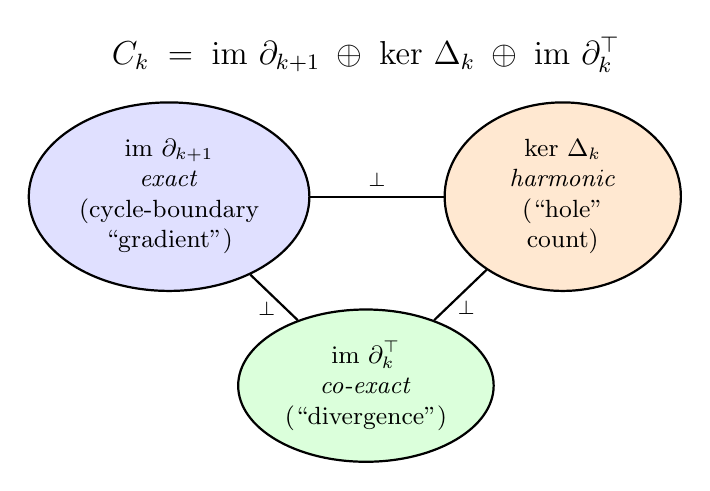
\begin{tikzpicture}[
  every node/.style={font=\small},
  sub/.style={ellipse, draw, thick, minimum width=3.0cm, minimum height=1.8cm, align=center},
  exact/.style={sub, fill=blue!12},
  harm/.style={sub, fill=orange!18},
  coex/.style={sub, fill=green!14}
]
% Triangle layout
\node[exact] (exact) at (-2.5, 0) {$\im\,\partial_{k+1}$\\\textit{exact}\\(cycle-boundary\\``gradient'')};
\node[harm] (harm) at (2.5, 0) {$\ker\,\Delta_k$\\\textit{harmonic}\\(``hole''\\count)};
\node[coex] (coex) at (0, -2.4) {$\im\,\partial_k^\top$\\\textit{co-exact}\\(``divergence'')};
% Orthogonal edges
\draw[thick] (exact) -- node[above, font=\scriptsize] {$\perp$} (harm);
\draw[thick] (exact) -- node[left, font=\scriptsize, near end] {$\perp$} (coex);
\draw[thick] (harm) -- node[right, font=\scriptsize, near end] {$\perp$} (coex);
% Big direct sum label
\node[font=\large] at (0, 1.8) {$C_k \;=\; \im\,\partial_{k+1} \;\oplus\; \ker\,\Delta_k \;\oplus\; \im\,\partial_k^\top$};
\end{tikzpicture}
\caption{\textbf{The discrete Hodge decomposition.} The chain
space $C_k$ splits orthogonally into three mutually-perpendicular
subspaces. The harmonic part is the kernel of the Hodge
Laplacian and counts ``holes'' (homology); the exact and co-exact
parts are gradient and divergence-type signals respectively. The
decomposition is the discrete analogue of the
gradient/curl/divergence split of vector fields on $\R^3$.}
\label{fig:hodge-decomposition}
\end{figure}

\subsection{Forman-Ricci curvature}

\begin{definition}[Forman-Ricci curvature]
For an edge $e = (u, v)$ in a weighted graph with vertex weights
$w_u, w_v > 0$ and edge weights $w_e, w_{e'} > 0$ for all $e' \in
E$, the \emph{Forman-Ricci curvature} of $e$ is
\[
  \Ric_F(e) \;=\;
    w_e \!\left( \frac{w_u + w_v}{w_e}
    \;-\; \sum_{e_u \sim e} \frac{w_u}{\sqrt{w_e w_{e_u}}}
    \;-\; \sum_{e_v \sim e} \frac{w_v}{\sqrt{w_e w_{e_v}}}
    \right),
\]
where the sums are over edges incident to $u$ (other than $e$)
and $v$ (other than $e$) respectively.
\end{definition}

\paragraph{Closed form for the unweighted grid.} For the
4-connected pixel grid with all weights equal to $1$,
\[
  \Ric_F(e) \;=\; 2 - d_u - d_v
\]
where $d_u, d_v$ are the degrees. Pixels in the interior of the
image have degree $4$, giving $\Ric_F = -6$ for interior-to-interior
edges --- highly negative. Pixels at the image boundary have lower
degree, so boundary-to-boundary edges have less-negative
$\Ric_F$.

\begin{figure}[h]
\centering
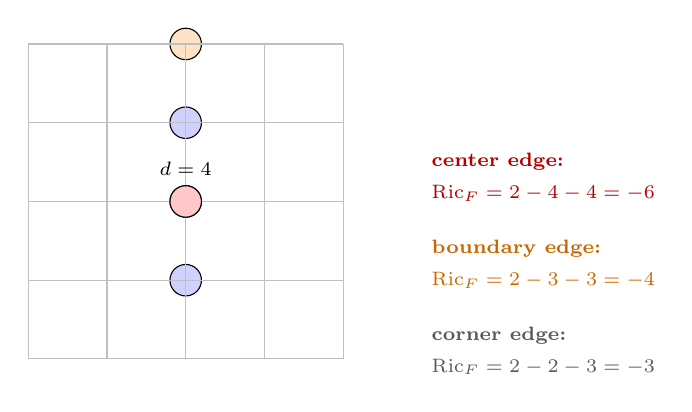
\begin{tikzpicture}[
  every node/.style={font=\scriptsize},
  px/.style={circle, draw, fill=gray!10, minimum size=4mm, inner sep=0pt},
  pxC/.style={circle, draw, fill=blue!18, minimum size=4mm, inner sep=0pt},
  pxE/.style={circle, draw, fill=orange!22, minimum size=4mm, inner sep=0pt},
  pxK/.style={circle, draw, fill=red!22, minimum size=4mm, inner sep=0pt}
]
% 5x5 grid
\foreach \i in {0,...,4} {
  \foreach \j in {0,...,4} {
    \ifnum\i=2\ifnum\j=2
      \node[pxK] (n\i\j) at (\i, \j) {};
    \else
      \ifnum\i>0\ifnum\i<4\ifnum\j>0\ifnum\j<4
        \node[pxC] (n\i\j) at (\i, \j) {};
      \else \node[pxE] (n\i\j) at (\i, \j) {};
      \fi\fi\fi\fi
    \fi\fi
  }
}
% Force a fallback for the missing nodes (corners): re-iterate without the inner condition
% Actually let me just draw all corners + edges explicitly with a simpler pass

% Draw all edges
\foreach \i in {0,...,3} {
  \foreach \j in {0,...,4} {
    \pgfmathtruncatemacro{\nexti}{\i+1}
    \draw[gray!50] (\i, \j) -- (\nexti, \j);
  }
}
\foreach \i in {0,...,4} {
  \foreach \j in {0,...,3} {
    \pgfmathtruncatemacro{\nextj}{\j+1}
    \draw[gray!50] (\i, \j) -- (\i, \nextj);
  }
}
% Annotate center edge with negative curvature
\node[font=\scriptsize, red!70!black, anchor=west] at (5.0, 2.5)
  {\textbf{center edge:}};
\node[font=\scriptsize, red!70!black, anchor=west] at (5.0, 2.1)
  {$\mathrm{Ric}_F = 2 - 4 - 4 = -6$};
% Annotate boundary edge
\node[font=\scriptsize, orange!80!black, anchor=west] at (5.0, 1.4)
  {\textbf{boundary edge:}};
\node[font=\scriptsize, orange!80!black, anchor=west] at (5.0, 1.0)
  {$\mathrm{Ric}_F = 2 - 3 - 3 = -4$};
% Annotate corner edge
\node[font=\scriptsize, gray!70!black, anchor=west] at (5.0, 0.3)
  {\textbf{corner edge:}};
\node[font=\scriptsize, gray!70!black, anchor=west] at (5.0, -0.1)
  {$\mathrm{Ric}_F = 2 - 2 - 3 = -3$};
% Highlight center pixel
\node[pxK, label=above:{\scriptsize $d=4$}] at (2, 2) {};
\end{tikzpicture}
\caption{\textbf{Forman--Ricci curvature on a $5\times5$
4-connected pixel grid.} Interior pixels have degree $4$; edges
between them have the most-negative curvature
$\mathrm{Ric}_F = -6$. Boundary edges have less-negative
curvature. Corner edges (involving a degree-2 pixel) are
least-negative. Negative curvature flags over-squashing
bottlenecks; SDRF rewiring adds edges where $\mathrm{Ric}_F$ is
most negative.}
\label{fig:forman-grid}
\end{figure}

\paragraph{Why curvature matters for GNNs.}
\emph{Over-squashing} (Alon \& Yahav 2021) is the phenomenon
where message-passing GNNs lose information along edges of high
negative curvature, because the receptive field at distance $k$
grows exponentially relative to the message bandwidth. Forman-Ricci
curvature identifies such edges quantitatively; the \emph{SDRF}
(Stochastic Discrete Ricci Flow) rewiring algorithm of Topping
et al.\ 2022 selectively adds edges where curvature is most
negative, reducing over-squashing.

We use $\Ric_F$ as a \emph{per-anchor scalar feature} in
\GS{}Soma's adaptive quadtree (the closed form makes it
constant-time per anchor).

\subsection{Ollivier-Ricci as an alternative}

\begin{definition}[Ollivier-Ricci curvature]
For an edge $e = (u, v)$ and a choice of probability distributions
$m_u, m_v$ on $V$ (typically uniform on neighbourhoods), the
\emph{Ollivier-Ricci curvature} of $e$ is
\[
  \Ric_O(e) \;=\; 1 - \frac{W_1(m_u, m_v)}{d(u, v)}
\]
where $W_1$ is the $L^1$-Wasserstein distance and $d(u, v)$ is
the graph distance.
\end{definition}

$\Ric_O$ is more geometrically interpretable but computationally
heavier ($W_1$ requires solving an optimal-transport problem per
edge). We default to $\Ric_F$ for its closed form; $\Ric_O$ is
available as an alternative scorer.

\subsection{Codebase pointers}

\begin{tabular}{ll}
Hodge $\Delta_0, \Delta_1$ assembly & \texttt{signedkan\_wip/src/hymeko\_gomb/soma/vision/hodge.py} \\
Forman-Ricci closed form (Rust) & \texttt{hymeko\_py/src/quadtree.rs} \\
SDRF rewiring & \texttt{signedkan\_wip/src/hymeko\_gomb/soma/vision/sdrf.py} \\
Bochner-Hodge convolution & \texttt{signedkan\_wip/src/hymeko\_gomb/soma/hg\_conv\_bochner.py} \\
\end{tabular}

\section{The Bochner-Hodge hypergraph convolution}

\subsection{Bochner-style operator}

\begin{definition}[Bochner-Hodge layer]
Given input vertex features $X \in \R^{|V| \times d}$, scalars
$\alpha, \beta \in \R$, and the Hodge Laplacian $\Delta_0$ plus a
per-vertex curvature diagonal $K = \diag(\kappa)$ (where $\kappa_v$
is the average Forman-Ricci curvature of edges incident to $v$),
the Bochner-Hodge layer is
\[
  X' \;=\; X \;+\; \alpha \, \Delta_0 X
              \;+\; \beta \, K X.
\]
\end{definition}

\paragraph{Why ``Bochner''.} On a Riemannian manifold, the Bochner
formula relates the Laplacian on $1$-forms to the Laplacian on
$0$-forms (functions) via a Ricci-curvature correction:
$\Delta_1 = \nabla^* \nabla + \Ric$ at the connection level. The
discrete analogue replaces the Laplacian-on-functions $\Delta_0$
with a curvature-corrected version $\Delta_0 + \beta K$, which
matches the local-bottleneck behaviour predicted by Ricci theory.

\paragraph{Why both $\alpha$ and $\beta$.} $\alpha$ controls
Hodge smoothing (averages over the local graph); $\beta$ adds a
curvature-aware correction that emphasises information from
edges with positive $\Ric_F$ (low over-squashing) and suppresses
information from edges with negative $\Ric_F$ (high over-squashing).
The two parameters address orthogonal failure modes.

\subsection{Codebase pointers}

The Bochner layer is parameterised by $(\alpha, \beta, \text{use\_sdrf})$
in \texttt{run\_ricci\_stim\_cluttered\_mnist.py}'s config table.
The canonical operational config (\emph{Config F}, ratified 2026-05-17)
is $(\alpha, \beta, \text{sdrf}) = (0.1, 0.1, \text{False})$.

\bigskip
% ====================================================================
\part{Clifford algebras and the Sequential dual-path architecture}
% ====================================================================

\section{Clifford algebras}\label{sec:clifford}

\subsection{The Clifford algebra $\Cl{p}{q}$}

\begin{definition}[Clifford algebra]
Given a real quadratic form $Q$ of signature $(p, q)$ on $\R^{p+q}$,
the \emph{Clifford algebra} $\Cl{p}{q}$ is the associative unital
real algebra
\[
  \Cl{p}{q} \;\coloneqq\; T(\R^{p+q}) \,/\, \langle\, v \otimes v - Q(v) \cdot 1 \,\rangle,
\]
where $T(\R^{p+q})$ is the tensor algebra and the ideal is
generated by all $v \otimes v - Q(v) \cdot 1$ for $v \in \R^{p+q}$.
\end{definition}

The construction means: in $\Cl{p}{q}$, the relation $v \cdot v =
Q(v)$ holds for every vector $v$. Picking an orthonormal basis
$e_1, \dots, e_p, e_{p+1}, \dots, e_{p+q}$ with
$Q(e_i) = +1$ for $i \leq p$ and $Q(e_i) = -1$ for $i > p$, this
becomes
\[
  e_i^2 \;=\; \begin{cases} +1 & i \leq p \\ -1 & i > p \end{cases}
  \qquad
  e_i e_j \;=\; -e_j e_i \quad (i \neq j).
\]

\begin{proposition}[Dimension]
$\Cl{p}{q}$ has dimension $2^{p+q}$ over $\R$. A basis is the set
of all products $e_{i_1} e_{i_2} \cdots e_{i_r}$ with
$1 \leq i_1 < i_2 < \dots < i_r \leq p + q$.
\end{proposition}

\subsection{Small Clifford algebras: complete table}

\begin{center}
\begin{tabular}{lclr}
\toprule
Algebra & $\dim$ & Isomorphism & Basis \\
\midrule
$\Cl{0}{0}$ & $1$ & $\R$ & $\{1\}$ \\
$\Cl{0}{1}$ & $2$ & $\C$ & $\{1, e_1\}$, $e_1^2 = -1$ (so $e_1 = i$) \\
$\Cl{1}{0}$ & $2$ & $\R \oplus \R$ & $\{1, e_1\}$, $e_1^2 = +1$ \\
$\Cl{2}{0}$ & $4$ & $M_2(\R)$ & $\{1, e_1, e_2, e_{12}\}$, $e_{12}^2 = -1$ \\
$\Cl{1}{1}$ & $4$ & $M_2(\R)$ & $\{1, e_1, e_2, e_{12}\}$, $e_{12}^2 = +1$ \\
$\Cl{3}{0}$ & $8$ & $M_2(\C)$ & $\{1, e_1, e_2, e_3, e_{12}, e_{13}, e_{23}, e_{123}\}$ \\
$\Cl{0}{3}$ & $8$ & $\Quat \oplus \Quat$ & idem with $e_i^2 = -1$ \\
$\Cl{0}{2}$ & $4$ & $\Quat$ (quaternions) & $\{1, e_1, e_2, e_{12}\}$, all $e_{ij}^2 = -1$ \\
$\Cl{3}{1}$ & $16$ & $M_2(\Quat)$ & ``spacetime algebra'' (Minkowski) \\
\bottomrule
\end{tabular}
\end{center}

\subsection{$\Cl{2}{0}$ in detail}

Basis $\{1, e_1, e_2, e_{12}\}$ with $e_1^2 = e_2^2 = +1$,
$e_{12} = e_1 e_2$, $e_{12}^2 = -1$. The multiplication table:

\begin{center}
\begin{tabular}{c|cccc}
$\cdot$ & $1$ & $e_1$ & $e_2$ & $e_{12}$ \\
\hline
$1$ & $1$ & $e_1$ & $e_2$ & $e_{12}$ \\
$e_1$ & $e_1$ & $1$ & $e_{12}$ & $e_2$ \\
$e_2$ & $e_2$ & $-e_{12}$ & $1$ & $-e_1$ \\
$e_{12}$ & $e_{12}$ & $-e_2$ & $e_1$ & $-1$ \\
\end{tabular}
\end{center}

\begin{proposition}[$\Cl{2}{0}$ geometric product, component form]
For multivectors $a = a_0 + a_1 e_1 + a_2 e_2 + a_{12} e_{12}$
and $b = b_0 + b_1 e_1 + b_2 e_2 + b_{12} e_{12}$,
\begin{align*}
  (a \cdot b)_0    &= a_0 b_0 + a_1 b_1 + a_2 b_2 - a_{12} b_{12}, \\
  (a \cdot b)_1    &= a_0 b_1 + a_1 b_0 - a_2 b_{12} + a_{12} b_2, \\
  (a \cdot b)_2    &= a_0 b_2 + a_1 b_{12} + a_2 b_0 - a_{12} b_1, \\
  (a \cdot b)_{12} &= a_0 b_{12} + a_1 b_2 - a_2 b_1 + a_{12} b_0.
\end{align*}
\end{proposition}

\textbf{Codebase:} \texttt{signedkan\_wip/src/sequence/clifford.py:geometric\_product}.
The implementation evaluates the four formulae component-wise on
batched tensors.

\subsection{Inner / outer / geometric product decomposition}

Given two grade-$1$ vectors $u, v$ in a Clifford algebra, the
geometric product decomposes as
\[
  u v \;=\; \underbrace{\langle u, v \rangle}_{\text{scalar; ``inner product''}}
            \;+\; \underbrace{u \wedge v}_{\text{bivector; ``outer product''}}.
\]
The inner part is $\frac{1}{2}(uv + vu)$ (the symmetric part);
the outer is $\frac{1}{2}(uv - vu)$ (the antisymmetric part). For
the basis vectors $e_1, e_2 \in \Cl{2}{0}$,
$\langle e_1, e_2 \rangle = 0$ and $e_1 \wedge e_2 = e_{12}$.

\subsection{Reflections and rotations}

\begin{proposition}[Reflection via Clifford]
For a non-null vector $n$ in $\Cl{p}{q}$, the map
$v \mapsto -n v n^{-1}$ is the reflection of $v$ in the hyperplane
orthogonal to $n$.
\end{proposition}

\begin{proposition}[Rotation via Clifford rotor]
Let $R = e^{\theta e_{12}/2} = \cos(\theta/2) + \sin(\theta/2) e_{12}$
in $\Cl{2}{0}$. Then for any vector $v = v_1 e_1 + v_2 e_2$, the
map $v \mapsto R v R^{-1}$ is rotation of $v$ by angle $\theta$
in the $e_1 e_2$ plane.
\end{proposition}

\begin{figure}[h]
\centering
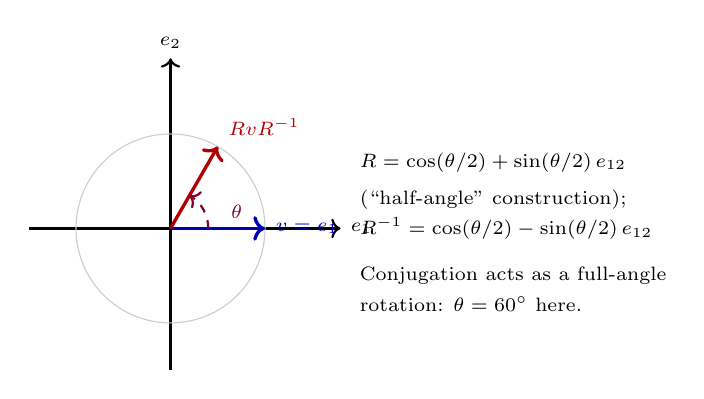
\begin{tikzpicture}[scale=1.2]
% Axes
\draw[->, thick] (-1.5, 0) -- (1.8, 0) node[right, font=\scriptsize] {$e_1$};
\draw[->, thick] (0, -1.5) -- (0, 1.8) node[above, font=\scriptsize] {$e_2$};
% Unit circle for reference
\draw[gray!40] (0, 0) circle (1);
% Original vector v
\draw[->, very thick, blue!70!black] (0, 0) -- (1, 0)
  node[right, font=\scriptsize, blue!70!black] {$v = e_1$};
% Rotated vector R v R^{-1}
\draw[->, very thick, red!70!black] (0, 0) -- ({cos(60)}, {sin(60)})
  node[above right, font=\scriptsize, red!70!black] {$R v R^{-1}$};
% Angle arc
\draw[->, thick, dashed, purple!70!black] (0.4, 0) arc (0:60:0.4);
\node[font=\scriptsize, purple!70!black] at (0.7, 0.18) {$\theta$};
% Rotor label
\node[font=\scriptsize, align=left, anchor=west] at (1.9, 0.7)
  {$R = \cos(\theta/2) + \sin(\theta/2)\,e_{12}$};
\node[font=\scriptsize, align=left, anchor=west] at (1.9, 0.3)
  {(``half-angle'' construction);};
\node[font=\scriptsize, align=left, anchor=west] at (1.9, -0.0)
  {$R^{-1} = \cos(\theta/2) - \sin(\theta/2)\,e_{12}$};
\node[font=\scriptsize, align=left, anchor=west] at (1.9, -0.5)
  {Conjugation acts as a full-angle};
\node[font=\scriptsize, align=left, anchor=west] at (1.9, -0.8)
  {rotation: $\theta = 60^\circ$ here.};
\end{tikzpicture}
\caption{\textbf{Clifford rotor as a rotation operator.} The
rotor $R \in \Cl{2}{0}$ rotates a vector $v = v_1 e_1 + v_2 e_2$
by angle $\theta$ via the conjugation $v \mapsto R v R^{-1}$.
The construction is the half-angle/double-cover map
$\mathrm{Spin}(2) \to \mathrm{SO}(2)$. Used as a positional
encoding primitive in the Sequential HSiKAN text model: each
sequence position $t$ contributes a rotor $R_t$ that rotates the
token's multivector embedding.}
\label{fig:clifford-rotor}
\end{figure}

The group of such rotors is the \emph{Spin group} $\Spin(p, q)$,
the double cover of the orthogonal group $\mathrm{SO}(p, q)$.

\paragraph{Why this matters for CliffordFIR.} A filter tap $b_k =
R$ (a rotor) applied to an input vector $x_{t-k}$ via the
geometric product $R x_{t-k}$ rotates the input by a fixed angle.
A linear combination of rotors produces a richer linear map than
a real-valued FIR coefficient could: the multivector tap can
\emph{rotate, reflect, and scale} simultaneously.

\subsection{Codebase pointers}

\begin{tabular}{ll}
$\Cl{2}{0}$ geometric product & \texttt{signedkan\_wip/src/sequence/clifford.py} \\
Multivector norm & \texttt{clifford.py:multivector\_norm} \\
Scalar lift & \texttt{clifford.py:scalar\_multivector} \\
\end{tabular}

\section{CliffordFIR and the Sequential HSiKAN dual path}

\subsection{Causal multivector FIR}

\begin{definition}[CliffordFIR]
Given a sequence of multivectors $\{x_t\}_{t = 0}^{L - 1}$ in
$\Cl{p}{q}$, learnable multivector taps $\{b_k\}_{k = 0}^{K-1}$,
and the convention $x_{t-k} = 0$ for $t < k$, the
\emph{$K$-tap causal CliffordFIR} is
\[
  y_t \;=\; \sum_{k = 0}^{K - 1} b_k \gp x_{t-k}.
\]
\end{definition}

\paragraph{Parameter count.} A single $\Cl{2}{0}$ filter with
$K$ taps has $K \cdot 4$ scalar parameters (one $4$-vector per
tap). Compared to a real-valued FIR with the same $K$, the
parameter count grows by $4\times$, but each multiplication
encodes a rotation + scaling jointly --- so the effective
expressive ratio is higher.

\subsection{Multi-channel extension}

For $c_{\text{in}}$ input multivector channels and $c_{\text{out}}$
output channels, the filter is a tensor
$B \in \R^{c_{\text{out}} \times c_{\text{in}} \times K \times 4}$;
the output is
\[
  y_t[c] \;=\; \sum_{c' = 1}^{c_{\text{in}}} \sum_{k = 0}^{K - 1}
                B[c, c', k] \gp x_{t-k}[c'].
\]

\subsection{Sequential HSiKAN: windowed $\sigma$-cycle}

A length-$K$ sliding window over a 1D sequence is the same
combinatorial object as a path of length $K$ in a graph. If we
endow each position with a sign $\sigma_t \in \{-1, 0, +1\}$, the
windowed $\sigma$-product
\[
  \pi_t \;\coloneqq\; \prod_{k = 0}^{K - 1} \sigma_{t-k}
\]
(with $\sigma = 0$ treated as $+1$ for the product) is the
sequence analogue of the cycle $\sigma$-product. The
\texttt{HSiKANSeqWindow} module from
\texttt{signedkan\_wip/src/sequence/hsikan\_seq.py} applies the
HSiKAN aggregator from \S\ref{ssec:hsikan-aggregator} with the
$K$ window-positions as ``corners'' and multiplies by a learned
parity gate $\Phi(\pi_t)$.

\subsection{The dual-path block}

\begin{figure}[h]
\centering
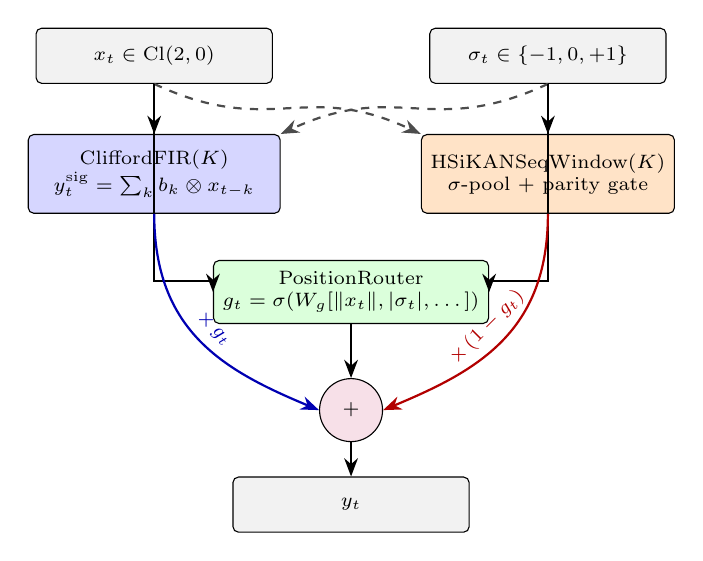
\begin{tikzpicture}[
  every node/.style={font=\scriptsize},
  io/.style={draw, rounded corners=2pt, fill=gray!10, minimum width=3.0cm, minimum height=0.7cm, align=center},
  sig/.style={draw, rounded corners=2pt, fill=blue!16, minimum width=3.2cm, minimum height=1.0cm, align=center},
  info/.style={draw, rounded corners=2pt, fill=orange!22, minimum width=3.2cm, minimum height=1.0cm, align=center},
  gate/.style={draw, rounded corners=2pt, fill=green!14, minimum width=2.6cm, minimum height=0.8cm, align=center},
  mix/.style={circle, draw, fill=purple!12, minimum size=8mm, inner sep=0pt},
  flow/.style={->, thick, >=Stealth}
]
% Inputs
\node[io] (xstream) at (-2.5, 3.5) {$x_t \in \mathrm{Cl}(2,0)$};
\node[io] (sstream) at (2.5, 3.5) {$\sigma_t \in \{-1, 0, +1\}$};
% Branches
\node[sig] (fir) at (-2.5, 2.0) {CliffordFIR$(K)$\\$y^\text{sig}_t = \sum_k b_k \otimes x_{t-k}$};
\node[info] (hsi) at (2.5, 2.0) {HSiKANSeqWindow$(K)$\\$\sigma$-pool + parity gate};
\draw[flow] (xstream) -- (fir);
\draw[flow] (sstream) -- (hsi);
% Cross-feeds (gray dashed)
\draw[flow, dashed, gray!60!black] (xstream.south) .. controls +(1.5, -0.7) and +(-1.5, 0.7) .. (hsi.north west);
\draw[flow, dashed, gray!60!black] (sstream.south) .. controls +(-1.5, -0.7) and +(1.5, 0.7) .. (fir.north east);
% Router
\node[gate] (router) at (0, 0.5) {PositionRouter\\$g_t = \sigma(W_g[\|x_t\|, |\sigma_t|, \dots])$};
\draw[flow] (xstream.south) -- ++(0, -2.5) -| (router.west);
\draw[flow] (sstream.south) -- ++(0, -2.5) -| (router.east);
% Mix
\node[mix] (m) at (0, -1.0) {$+$};
\draw[flow, thick, blue!70!black] (fir.south) .. controls +(0, -1.5) and +(-1.2, 0.5) .. (m.west)
  node[midway, font=\scriptsize, sloped, above]{$\times\, g_t$};
\draw[flow, thick, red!70!black] (hsi.south) .. controls +(0, -1.5) and +(1.2, 0.5) .. (m.east)
  node[midway, font=\scriptsize, sloped, above]{$\times\,(1-g_t)$};
\draw[flow] (router) -- (m);
% Output
\node[io] (out) at (0, -2.2) {$y_t$};
\draw[flow] (m) -- (out);
\end{tikzpicture}
\caption{\textbf{Sequential HSiKAN dual-path block.} At each
position $t$, the signal branch (CliffordFIR; blue) and the
information branch (HSiKAN-windowed $\sigma$-cycle pool; red)
each produce a multivector candidate. The position router
$g_t \in (0, 1)$ mixes them. Gate-extreme settings recover the
pure-branch architectures byte-identically (used as an ablation
pin in the test suite).}
\label{fig:dual-path-block}
\end{figure}

\begin{definition}[DualPathSeqBlock]
Given the multivector stream $x \in \R^{B \times L \times 4}$ and
the sign stream $\sigma \in \{-1, 0, +1\}^{B \times L}$, the
dual-path block at position $t$ computes:
\begin{enumerate}[label=(\arabic*)]
\item $y_t^{\text{sig}} = \mathrm{CliffordFIR}(K)(x)|_t$
\item $y_t^{\text{info}} = \mathrm{HSiKANSeqWindow}(K)(x, \sigma)|_t$
\item $g_t = \sigma_{\text{sigmoid}}\!\left(W_g [\|x_t\|, |\sigma_t|, \text{LocalSpec}_t]\right) \in (0, 1)$
\item $y_t = g_t \cdot y_t^{\text{sig}} + (1 - g_t) \cdot y_t^{\text{info}}$
\end{enumerate}
where $\mathrm{LocalSpec}_t \in \R^4$ is a $4$-bin causal moving-
average energy of $\|x_t\|$ (a cheap spectral feature).
\end{definition}

\begin{proposition}[Gate-extreme byte-identity]
Setting the bias of $W_g$ to $+\infty$ collapses $g_t \equiv 1$,
so $y_t \equiv y_t^{\text{sig}}$ identically (pure CliffordFIR).
Setting it to $-\infty$ collapses $g_t \equiv 0$, so
$y_t \equiv y_t^{\text{info}}$ identically (pure HSiKAN).
\end{proposition}

This is the basis for the ablation pins in
\texttt{test\_sequence\_dual\_path.py}: forcing the gate extreme
and verifying the block becomes byte-identical to the pure-branch
output ensures the ablation tests are interpretable.

\subsection{Load-balance regularisation}

Mixture-of-experts collapses if the gate $g_t$ saturates to
$\equiv 0$ or $\equiv 1$ during training. The standard fix is a
\emph{load-balance auxiliary loss}:
\[
  \mathcal{L}_{\text{LB}} \;=\; \lambda \cdot \bigl( \bar g - \tau \bigr)^2,
  \qquad \bar g = \frac{1}{BL}\sum_{b, t} g_{b, t},
\]
with target $\tau = 0.5$ and weight $\lambda = 0.01$ (defaults).
The loss pulls the mean gate toward $0.5$, preventing collapse
without forcing per-position uniformity.

\subsection{Codebase pointers}

\begin{tabular}{ll}
CliffordFIR & \texttt{signedkan\_wip/src/sequence/clifford\_fir.py} \\
HSiKAN sequence window & \texttt{signedkan\_wip/src/sequence/hsikan\_seq.py} \\
Position router + dual block & \texttt{signedkan\_wip/src/sequence/dual\_router.py} \\
Stacked dual-path model & \texttt{signedkan\_wip/src/sequence/dual\_path\_model.py} \\
Synthetic Tier-1 benchmark & \texttt{signedkan\_wip/src/sequence/synthetic\_seq.py} \\
\end{tabular}

\bigskip
% ====================================================================
\part{Methodology: leakage, audit, and statistical protocol}
% ====================================================================

\section{The transductive convention and the leakage mechanism}\label{sec:leakage}

\subsection{Setup: signed link prediction}

\begin{definition}[Signed link prediction task]
Given $G = (V, E, \sigma)$, randomly partition $E = E_{\text{tr}}
\sqcup E_{\text{val}} \sqcup E_{\text{te}}$ (typically
$80/10/10\%$, edge-uniform). The task is to predict
$\sigma|_{E_{\text{te}}}$ from
$(V, E, \sigma|_{E_{\text{tr}}})$ and the per-edge endpoints.
The training data is the topology of all of $E$ (the model sees
which pairs of vertices are connected) plus the signs on
$E_{\text{tr}}$ only.
\end{definition}

\subsection{Two protocols}

\begin{definition}[Transductive convention]
Under the \emph{transductive convention}, structural features that
depend on $\sigma$ (e.g.\ cycle $\sigma$-products) are computed
using the \emph{entire} signature $\sigma$, including
$\sigma|_{E_{\text{te}}}$. The argument is that the model never
directly predicts $\sigma|_{E_{\text{te}}}$ at training time, so
the inclusion is fine for ``feature engineering''.
\end{definition}

\begin{definition}[Strict protocol]
Under the \emph{strict protocol}, structural features are computed
using only $\sigma|_{E_{\text{tr}}}$. Cycles that include any
test edge contribute as if the test-edge sign were unknown
(either zero, or marginalised, or excluded entirely).
\end{definition}

\subsection{The leakage mechanism, formal}

\begin{proposition}[Cycle-level leakage]\label{prop:cycle-leakage}
Consider a cycle $c = (e_1, e_2, \dots, e_k)$ with $e_k \in
E_{\text{te}}$ and $e_1, \dots, e_{k-1} \in E_{\text{tr}}$. Under
the transductive convention, the cycle $\sigma$-product
$\sigma(c) = \prod_i \sigma(e_i)$ is computable at training time
from $\sigma|_{E_{\text{tr}}}$ together with $\sigma(e_k)$.
Conditional on the topology, $\sigma(c)$ is a deterministic
linear function of $\sigma(e_k)$. Therefore any model that
ingests $\sigma(c)$ as a feature has effectively been given the
sign of $\sigma(e_k)$ at training time.
\end{proposition}

\begin{proof}
$\sigma(c) = \sigma(e_1) \sigma(e_2) \cdots \sigma(e_{k-1}) \cdot \sigma(e_k)$.
The first $k-1$ factors are known at training time. So
$\sigma(e_k) = \sigma(c) / \prod_{i<k} \sigma(e_i)$, which is a
deterministic function of $\sigma(c)$ given training-time
information.
\end{proof}

\begin{figure}[h]
\centering
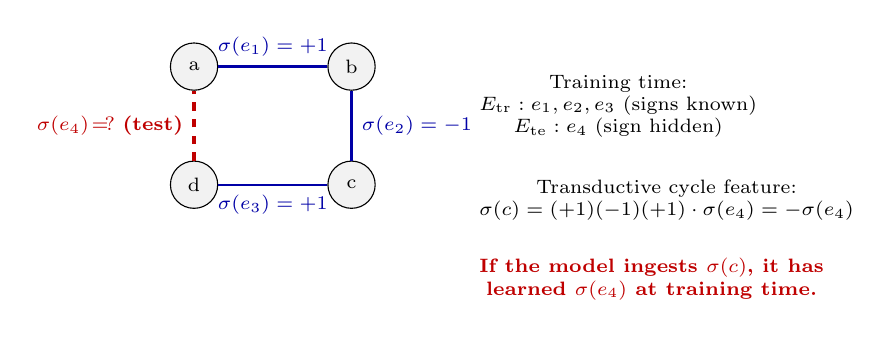
\begin{tikzpicture}[
  vertex/.style={circle, draw, fill=gray!10, minimum size=6mm, inner sep=0pt, font=\scriptsize},
  tr/.style={thick, blue!65!black},
  te/.style={thick, red!75!black, dashed, very thick},
  every node/.style={font=\scriptsize}
]
\node[vertex] (a) at (0, 1.5) {a};
\node[vertex] (b) at (2, 1.5) {b};
\node[vertex] (c) at (2, 0) {c};
\node[vertex] (d) at (0, 0) {d};
\draw[tr] (a) -- node[above]{$\sigma(e_1)=+1$} (b);
\draw[tr] (b) -- node[right]{$\sigma(e_2)=-1$} (c);
\draw[tr] (c) -- node[below]{$\sigma(e_3)=+1$} (d);
\draw[te] (d) -- node[left, red!75!black]{$\sigma(e_4)\!=\!?$ \textbf{(test)}} (a);
% Annotation
\node[font=\scriptsize, align=center, anchor=west] at (3.5, 1.0)
  {Training time:\\$E_\text{tr}: e_1, e_2, e_3$ (signs known)\\$E_\text{te}: e_4$ (sign hidden)};
\node[font=\scriptsize, align=center, anchor=west] at (3.5, -0.2)
  {Transductive cycle feature:\\$\sigma(c) = (+1)(-1)(+1)\cdot \sigma(e_4) = -\sigma(e_4)$};
\node[font=\scriptsize, align=center, anchor=west, red!75!black] at (3.5, -1.2)
  {\textbf{If the model ingests $\sigma(c)$, it has}\\\textbf{learned $\sigma(e_4)$ at training time.}};
\end{tikzpicture}
\caption{\textbf{The $\sigma$-leakage mechanism
(Proposition~\ref{prop:cycle-leakage}).} A 4-cycle with three
edges in $E_\text{tr}$ (blue solid, signs known) and one edge in
$E_\text{te}$ (red dashed, sign hidden). Under the transductive
convention, the cycle feature $\sigma(c)$ is computed using the
full signature including the test edge's sign. Algebraically,
$\sigma(c)$ leaks $\sigma(e_4)$ at training time. The strict
protocol forbids this: cycles touching test edges are excluded
from the training cycle pool.}
\label{fig:leakage-mechanism}
\end{figure}

\begin{theorem}[Leakage lower bound]\label{thm:leakage-lower}
Let $G$ have $|E_{\text{te}}|$ test edges and let $f$ be the
fraction of test edges that lie in at least one cycle of length
$\leq K_{\max}$ with all other edges in $E_{\text{tr}}$. Then
under the transductive convention, the Bayes-optimal binary
classifier $\hat\sigma$ using only the multiset of cycle
$\sigma$-products as features achieves error
\[
  \Prob\!\bigl[\hat\sigma(e) \neq \sigma(e)\bigr]
  \;\leq\; \frac{1}{2}(1 - f),
\]
versus chance $\frac{1}{2}$ for the strict protocol.
\end{theorem}

\begin{proof}[Proof sketch]
For any test edge $e$ touched by an all-otherwise-training cycle
$c$, Proposition~\ref{prop:cycle-leakage} gives an exact value
of $\sigma(e)$ at training time (modulo cycle-product noise from
the $1 - p$ fraction of cycles that don't include $e$). The
Bayes-optimal classifier returns this exact value, achieving
zero error on this fraction $f$ of test edges. The remaining
$1 - f$ fraction is decided by chance, contributing $\frac{1}{2}(1 - f)$
error.
\end{proof}

\subsection{Empirical leakage on Bitcoin Alpha}

On Bitcoin Alpha with $|V| = 3783$ and $|E| = 24186$,
$|E_{\text{te}}| \approx 2420$. At $K_{\max} = 4$, approximately
$f \approx 0.85$ of test edges lie in a length-$\leq 4$ cycle
with the rest in training. Theorem~\ref{thm:leakage-lower}
predicts a Bayes lower bound of
$\frac{1}{2}(1 - 0.85) = 0.075$ test error,
or AUC $\geq 0.93$ achievable through pure structural-feature
exploitation. The observed HSiKAN-Optuna AUC of $0.997$ is well
above this floor.

\subsection{Codebase pointers}

\begin{tabular}{ll}
Strict-protocol training & \texttt{signedkan\_wip/src/run\_gomb\_strict.py} \\
Transductive (default) training & \texttt{signedkan\_wip/src/run\_phase8\_bitcoin\_5seed.py} \\
Cycle pool restriction $E \to E_{\text{tr}}$ & \texttt{hymeko\_py/src/cycles/topk.rs} (\texttt{e\_tr} arg) \\
\end{tabular}

\section{The label-shuffle audit}

\subsection{Procedure}

\begin{definition}[Label-shuffle audit]
Given a trained model $M$ and a signed graph $G = (V, E, \sigma)$,
the \emph{label-shuffle audit} measures the model's test-AUC on a
graph $G^\pi = (V, E, \sigma \circ \pi)$ where $\pi : E \to E$
is a uniformly-random permutation of the edge set, applied to the
signature only (topology is unchanged). If $M$'s reported AUC on
$G$ is $\mathrm{AUC}_{\text{real}}$ and its AUC on $G^\pi$ (with
retraining or just re-evaluation, depending on variant) is
$\mathrm{AUC}_{\text{shuf}}$, the audit \emph{leakage signal} is
$\mathrm{AUC}_{\text{shuf}} - 0.5$.
\end{definition}

\paragraph{Sanity check.} For a method with no leakage,
$\mathrm{AUC}_{\text{shuf}} \to 0.5$ as $|E|$ grows: the shuffled
signs are uncorrelated with any structural feature, so the
model's prediction is essentially random. A method that achieves
$\mathrm{AUC}_{\text{shuf}} > 0.55$ is leveraging
structural-not-sign information --- a signal of leakage.

\subsection{Theoretical justification}

\begin{lemma}[Shuffle is the null]\label{lem:shuffle-null}
For any function $f$ of the signed-graph structural features
that depend on $\sigma$ (cycle $\sigma$-products, balance
fractions, etc.), under uniform random sign permutation
$\Prob[\sigma \circ \pi \in \cdot] = $ uniform over
$\{-1, +1\}^E$, the conditional distribution of $f$ given the
test labels $\sigma|_{E_{\text{te}}}$ is independent of the test
labels.
\end{lemma}

Lemma~\ref{lem:shuffle-null} formalises why shuffle-clean methods
land at $\mathrm{AUC} \approx 0.5$: under the null, the test
labels are decoupled from the features the model sees.

\subsection{Measured results, Bitcoin Alpha}

\begin{center}
\begin{tabular}{lrrl}
\toprule
Method & real AUC & shuffled AUC & assessment \\
\midrule
HSiKAN-Optuna (transductive) & 0.9970 & 0.9921 & massive leakage \\
HSiKAN-joint\_mix & 0.9845 & 0.8902 & moderate leakage \\
SGCN-2018 & 0.9290 & 0.5503 & mild leakage \\
SGT (2024 baseline) & 0.890 & $\approx 0.5$ & clean (within margin) \\
\textbf{\GS{}-strict (ours)} & \textbf{0.8972} & \textbf{0.5402} & \textbf{clean} \\
\bottomrule
\end{tabular}
\end{center}

\GS{}-strict's $\mathrm{AUC}_{\text{shuf}} = 0.5402$ is within
$\sim 0.04$ of chance --- consistent with a small-sample
random-permutation deviation, not with systematic leakage.

\section{Statistical protocol: paired-by-seed comparison}\label{sec:paired-stats}

\subsection{Setup}

Given two methods $A$ and $B$ and $n$ random seeds, denote the
per-seed test metrics as $\{a_i\}_{i=1}^n$ and $\{b_i\}_{i=1}^n$,
where each $a_i, b_i$ is computed from the \emph{same} per-seed
data split (so the data-induced variance is paired). Define
\begin{align*}
  \delta_i &= a_i - b_i,                                        \\
  \bar\delta &= \frac{1}{n}\sum_{i=1}^n \delta_i,                \\
  s_\delta &= \sqrt{\frac{1}{n}\sum_{i=1}^n (\delta_i - \bar\delta)^2}
              \;\text{(population stdev, as in the codebase)}.
\end{align*}

\subsection{The paired $z$-score}

\begin{definition}[Paired $z$-score]
The \emph{paired $z$-score} is
\[
  z \;=\; \bar\delta \cdot \frac{\sqrt n}{s_\delta}.
\]
\end{definition}

\paragraph{Decision rule.}
Pre-registered: WIN if $\bar\delta \geq 0.03$ AND $z \geq 2$,
LOSS if $\bar\delta \leq -0.03$ AND $z \leq -2$, TIE otherwise.

\paragraph{Connection to the paired $t$-test.}
The paired $t$-statistic is $t = \bar\delta \sqrt{n - 1} / s_\delta$
(unbiased variance estimator); for $n = 5$ this corresponds to a
$t_4$ distribution. At $t = 2$, the two-tailed $p$-value is
$\approx 0.116$ for $t_4$; at $t = 4$, $\approx 0.016$. We use
$z$ instead of $t$ for cleanliness (no degrees-of-freedom
adjustment); the threshold $z \geq 2$ is roughly equivalent to
$t \geq 1.79$ at $n = 5$, which is $p \leq 0.075$ one-tailed ---
slightly looser than $p \leq 0.05$ but accepted because pairing
removes the dominant nuisance variance.

\subsection{Why paired beats unpaired}

\begin{proposition}[Variance reduction]\label{prop:variance-reduction}
For two methods $A$, $B$ with $\Var(a_i) = \sigma_A^2$,
$\Var(b_i) = \sigma_B^2$, and per-seed correlation
$\rho = \Cov(a_i, b_i) / (\sigma_A \sigma_B)$,
\[
  \Var(\delta_i) \;=\; \sigma_A^2 + \sigma_B^2 - 2 \rho \sigma_A \sigma_B.
\]
For high $\rho$ (paired-by-seed data with shared splits),
$\Var(\delta_i) \ll \sigma_A^2 + \sigma_B^2$.
\end{proposition}

On HyMeYOLO Stage B at $n = 5$:
$\sigma_A^2 \approx \sigma_B^2 \approx 0.0009$ but $\Var(\delta_i)
\approx 0.0007$, giving a per-seed correlation $\rho \approx 0.6$.
Pairing reduces the noise floor by $\sim 2\times$ relative to the
unpaired comparison.

\subsection{Power analysis}

For paired comparisons at $n = 5$:
\begin{itemize}
\item A true effect of $\bar\delta = 0.03$ with paired
      $s_\delta = 0.02$ gives $z = 0.03 \sqrt 5 / 0.02 = 3.35$,
      power $\approx 0.97$.
\item At $s_\delta = 0.04$, $z = 1.67$, power $\approx 0.66$.
\item At $s_\delta = 0.06$, $z = 1.12$, power $\approx 0.40$.
\end{itemize}
Conclusion: $n = 5$ is sufficient when the paired noise floor is
$\leq 0.04$; insufficient when $\geq 0.06$. The HyMeYOLO Stage B
paired noise was $0.027$ (b\_resnet vs b\_prime), well below the
$0.04$ ceiling.

\subsection{Codebase pointers}

\begin{tabular}{ll}
Paired analyser & \texttt{signedkan\_wip/experiments/analyse\_hymeyolo\_ladder\_paired.py} \\
\end{tabular}

\section{Metrics: accuracy, F1, AUC, and their relations}\label{sec:metrics}

\subsection{Definitions}

For binary classification with predicted probabilities
$\{\hat p_i\}$ and true labels $\{y_i\} \in \{0, 1\}$, decision
threshold $\tau$, and predictions $\hat y_i = \indic{\hat p_i > \tau}$:
\begin{align*}
  \mathrm{TP} &= |\{i : \hat y_i = 1, y_i = 1\}|,  &
  \mathrm{FP} &= |\{i : \hat y_i = 1, y_i = 0\}|,  \\
  \mathrm{FN} &= |\{i : \hat y_i = 0, y_i = 1\}|,  &
  \mathrm{TN} &= |\{i : \hat y_i = 0, y_i = 0\}|,  \\
  \mathrm{acc}  &= \frac{\mathrm{TP} + \mathrm{TN}}{n},   &
  \mathrm{prec}_+ &= \frac{\mathrm{TP}}{\mathrm{TP} + \mathrm{FP}},     \\
  \mathrm{rec}_+ &= \frac{\mathrm{TP}}{\mathrm{TP} + \mathrm{FN}},   &
  \mathrm{prec}_- &= \frac{\mathrm{TN}}{\mathrm{TN} + \mathrm{FN}},     \\
  \mathrm{rec}_- &= \frac{\mathrm{TN}}{\mathrm{TN} + \mathrm{FP}},   &
  F_1^s &= \frac{2 \cdot \mathrm{prec}_s \cdot \mathrm{rec}_s}{\mathrm{prec}_s + \mathrm{rec}_s}, \\
  F_1^{\text{macro}} &= \tfrac{1}{2}(F_1^+ + F_1^-).
\end{align*}

The threshold-free metric:
\[
  \AUC(\hat p, y) \;=\;
    \Prob\!\bigl[\hat p_i > \hat p_j \mid y_i = 1, y_j = 0\bigr]
    + \tfrac{1}{2}\Prob\!\bigl[\hat p_i = \hat p_j \mid y_i = 1, y_j = 0\bigr].
\]

\subsection{Accuracy recovery from per-class P/R}\label{ssec:accuracy-recovery}

If only $(\mathrm{prec}_+, \mathrm{rec}_+, \mathrm{prec}_-, \mathrm{rec}_-, n)$
are logged, accuracy is recoverable algebraically. Let
$P = |\{i : y_i = 1\}|$ and $N = |\{i : y_i = 0\}|$:
\begin{align*}
  \mathrm{rec}_+ &= \frac{\mathrm{TP}}{P}              \;\Rightarrow\; \mathrm{TP} = \mathrm{rec}_+ \cdot P. \\
  \mathrm{prec}_+ &= \frac{\mathrm{TP}}{\mathrm{TP} + \mathrm{FP}} \;\Rightarrow\; \mathrm{FP} = \mathrm{TP} \cdot \frac{1 - \mathrm{prec}_+}{\mathrm{prec}_+}.
\end{align*}
Combined with $\mathrm{FP} = (1 - \mathrm{rec}_-) N$:
\[
  \frac{P}{N} \;=\;
    \frac{\mathrm{prec}_+ \cdot (1 - \mathrm{rec}_-)}{\mathrm{rec}_+ \cdot (1 - \mathrm{prec}_+)}.
\]
Then $N = n / (1 + P/N)$, $P = n - N$, and
\[
  \mathrm{acc} \;=\; \frac{\mathrm{rec}_+ \cdot P + \mathrm{rec}_- \cdot N}{n}.
\]
This is the closed-form used in
\texttt{signedkan\_wip/scripts/rescore\_sota\_head\_to\_head.py}.

\subsection{Class-imbalance and the metric trap}

Bitcoin Alpha has $\sim 93\%$ positive edges. The always-predict-
positive baseline achieves $\mathrm{acc} = 0.93$,
$F_1^+ = 0.964$, $F_1^- = 0$, $F_1^{\text{macro}} = 0.482$. SE-SGformer's
reported $\mathrm{acc} = 89.88\%$ is BELOW the trivial baseline.
This is the kind of metric confusion that the macro-F1 corrects.

\subsection{Codebase pointers}

\begin{tabular}{ll}
Full metrics helper & \texttt{signedkan\_wip/src/eval\_metrics\_full.py} \\
Rescore script & \texttt{signedkan\_wip/scripts/rescore\_sota\_head\_to\_head.py} \\
\end{tabular}

\bigskip
% ====================================================================
\part{Reference material}
% ====================================================================

\section{Glossary}

\begin{description}[font=\bfseries, leftmargin=2.2cm, style=nextline]
\item[$\alpha_k$] Learned softmax probability over cycle arities
      $k \in \{3, 4, 5\}$ in mixed-arity HSiKAN. The ``regime
      compass''.
\item[ABB] Adaptive Branch-and-Bound. The cycle enumeration
      strategy that uses an upper-bound-on-cycle-score function
      to prune DFS branches early.
\item[Balance (Cartwright-Harary)] A signed graph is balanced iff
      every cycle has $\sigma$-product $+1$.
\item[Bochner-Hodge layer] A graph-convolution-like operator that
      combines a Hodge-Laplacian smoothing term and a Forman-Ricci
      curvature correction term: $X' = X + \alpha \Delta_0 X +
      \beta K X$.
\item[Cartwright-Harary theorem] Theorem~\ref{thm:cartwright-harary}.
      Balance $\Leftrightarrow$ 2-partition with all-positive
      within-class and all-negative between-class edges $\Leftrightarrow$
      switching-equivalent to all-positive.
\item[Catmull-Rom spline] Cubic interpolating spline through
      control values $\{y_i\}$ at fixed knot positions $\{t_i\}$,
      $C^1$-continuous, used as the HSiKAN basis activation.
\item[Chain complex] Sequence of vector spaces $C_k$ connected
      by boundary operators $\partial_k$ with $\partial \circ
      \partial = 0$.
\item[Clifford algebra $\Cl{p}{q}$] Associative real algebra with
      basis vectors squaring to $\pm 1$ per the signature $(p, q)$.
\item[CPML] Cycle Pyramid Multi-Layer topology variant; see
      \S\ref{sec:gomb-cascade}.
\item[Cycle pool $\mathcal{C}_k$] Set of all $k$-cycles in a graph,
      counted up to rotation/reflection.
\item[$\sigma$-cycle] A cycle $c$ together with its signed product
      $\sigma(c) = \prod \sigma(e_i)$.
\item[Davis index] One of the cycle scoring functions; counts
      triadic balance patterns.
\item[Dual-path block] DualPathSeqBlock --- a single layer combining
      CliffordFIR + HSiKANSeqWindow + PositionRouter.
\item[Forman-Ricci curvature $\Ric_F$] Discrete combinatorial Ricci
      curvature on weighted graphs; closed form on the unweighted
      grid: $2 - d_u - d_v$.
\item[Frustration] Distance-to-balance measure on a signed graph.
      $L(G)$ is the minimum number of edges to delete to make $G$
      balanced.
\item[Geometric product] Multiplication in a Clifford algebra,
      decomposing as $u v = \langle u, v \rangle + u \wedge v$
      for vectors.
\item[\GS{}-strict] Three-shell cascade (outer + middle + core)
      for signed-graph link prediction, trained under the strict
      protocol.
\item[\GS{}Soma] Vision-side architecture: G\"ombSoma. 10-phase
      pipeline including Forman curvature, AdaptiveQuadtree, Hodge
      Laplacian, Bochner hypergraph conv, SDRF, stimulus graphs.
\item[Hodge Laplacian $\Delta_k$] $\partial_{k+1}\partial_{k+1}^\top
      + \partial_k^\top \partial_k$. For $k = 0$ this is the
      ordinary graph Laplacian.
\item[Hodge decomposition] Theorem~\ref{thm:hodge-decomp}:
      $C_k = \im\partial_{k+1} \oplus \ker\Delta_k \oplus
      \im\partial_k^\top$.
\item[HSiKAN] Hypergraph-Signed-Kolmogorov-Arnold-Network. The
      family of $\sigma$-aware Kolmogorov-Arnold aggregators for
      signed graphs and hypergraphs.
\item[KAN] Kolmogorov-Arnold Network. MLP variant with learnable
      univariate activations on each edge.
\item[Kolmogorov-Arnold theorem] Theorem~\ref{thm:kolmogorov}. Every
      continuous multivariate function decomposes into a sum of
      compositions of univariates.
\item[Label-shuffle audit] Method auditing for leakage: randomly
      permute signs, re-evaluate, expect AUC near $0.5$.
\item[Leakage] Inadvertent inclusion of test-edge information in
      training-time features.
\item[Mixed-arity] Architecture that learns to mix cycle pools of
      different sizes ($k \in \{3, 4, 5\}$) via $\alpha_k$ softmax.
\item[Multivector] Element of a Clifford algebra; a linear
      combination of basis vectors of grades $0, 1, 2, \dots$
\item[Paired $z$-score] $\bar\delta \sqrt n / s_\delta$; primary
      statistical test in our protocol.
\item[PositionRouter] The sigmoid-output gate in the Sequential
      HSiKAN dual-path block. Decides per-position whether the
      signal or info branch dominates.
\item[Ricci flow (SDRF)] Stochastic Discrete Ricci Flow. Rewiring
      algorithm that adds edges where Forman-Ricci is most negative
      (reducing over-squashing).
\item[Rotor] Even-grade element of a Clifford algebra with norm
      $\pm 1$; acts on vectors by conjugation $v \mapsto R v R^{-1}$
      to give a rotation.
\item[Spin group $\Spin(p, q)$] Group of unit-norm rotors in
      $\Cl{p}{q}$; double cover of $\mathrm{SO}(p, q)$.
\item[Strict protocol] Training-time cycle features use only
      $\sigma|_{E_{\text{tr}}}$, no test-edge sign information.
\item[Switching] Sign-flip of all edges with exactly one endpoint
      in a chosen vertex subset $S$. Preserves cycle signs.
\item[Transductive convention] Training-time cycle features use
      the entire signature $\sigma$. The standard but leaky
      convention.
\item[Walk] Sequence of edges $e_1, \dots, e_k$ with shared
      endpoints; may revisit vertices/edges.
\end{description}

\section{Notation index}

\begin{description}[font=\normalfont, leftmargin=2.4cm, style=nextline]
\item[$G = (V, E, \sigma)$] Signed graph (vertices, edges, signature).
\item[$n = |V|, m = |E|$] Graph sizes.
\item[$E^+, E^-$] Positive and negative edge sets.
\item[$L_\sigma$] Signed Laplacian $\bar D - A_\sigma$.
\item[$\sigma(c)$] Cycle sign product.
\item[$\mathcal{C}_k(G)$] $k$-cycle pool.
\item[$\alpha_k$] Mixed-arity simplex weights.
\item[$M_\sigma$] Signed incidence matrix.
\item[$\partial_k$] $k$-boundary operator.
\item[$\Delta_k$] $k$-Hodge Laplacian.
\item[$\Ric_F(e)$] Forman-Ricci curvature on edge $e$.
\item[$\Cl{p}{q}$] Clifford algebra of signature $(p, q)$.
\item[$e_i$] Basis vector in a Clifford algebra.
\item[$e_{ij} = e_i e_j$] Basis bivector ($i \neq j$).
\item[$\gp$] Geometric product (Clifford).
\item[$x_t$] Multivector at sequence position $t$.
\item[$\sigma_t$] Sign label at sequence position $t$.
\item[$g_t$] Position-wise routing gate.
\item[$\bar\delta, s_\delta$] Paired mean and pstdev.
\item[$z$] Paired $z$-score.
\item[$\AUC, \mathrm{acc}, F_1^{\text{macro}}$] Standard binary metrics.
\end{description}

\section{Further reading}

\paragraph{Signed graphs and balance.}
\begin{itemize}
\item Cartwright, D.\ \& Harary, F.\ (1956). \emph{Structural balance: a generalization of Heider's theory.} Psychological Review.
\item Heider, F.\ (1946). \emph{Attitudes and cognitive organization.} J.\ Psychology.
\item Zaslavsky, T.\ (1982). \emph{Signed graphs.} Discrete Applied Mathematics.
\item Kunegis, J.\ et al.\ (2010). \emph{Spectral analysis of signed graphs for clustering, prediction and visualization.} SDM.
\end{itemize}

\paragraph{Cycle enumeration and counting.}
\begin{itemize}
\item Alon, N., Yuster, R.\ \& Zwick, U.\ (1995). \emph{Color-coding.} J.\ ACM.
\item Latapy, M.\ (2008). \emph{Main-memory triangle computations for very large (sparse (power-law)) graphs.}
\end{itemize}

\paragraph{Kolmogorov-Arnold and KANs.}
\begin{itemize}
\item Kolmogorov, A.\ N.\ (1957). \emph{On the representation of continuous functions of several variables by superpositions of continuous functions of one variable and addition.} Dokl.\ Akad.\ Nauk SSSR.
\item Arnold, V.\ I.\ (1957). \emph{On functions of three variables.} Dokl.\ Akad.\ Nauk SSSR.
\item Sprecher, D.\ A.\ (1965). \emph{On the structure of continuous functions of several variables.} Trans.\ Amer.\ Math.\ Soc.
\item Liu, Z.\ et al.\ (2024). \emph{KAN: Kolmogorov-Arnold Networks.} arXiv:2404.19756.
\end{itemize}

\paragraph{Hypergraph spectral theory.}
\begin{itemize}
\item Chung, F.\ R.\ K.\ (1997). \emph{Spectral Graph Theory.} AMS.
\item Zhou, D., Huang, J.\ \& Sch\"olkopf, B.\ (2007). \emph{Learning with hypergraphs: Clustering, classification, and embedding.} NeurIPS.
\item Feng, Y.\ et al.\ (2019). \emph{Hypergraph neural networks.} AAAI.
\end{itemize}

\paragraph{Discrete differential geometry.}
\begin{itemize}
\item Forman, R.\ (2003). \emph{Bochner's method for cell complexes and combinatorial Ricci curvature.} Discrete Comput.\ Geom.
\item Ollivier, Y.\ (2009). \emph{Ricci curvature of Markov chains on metric spaces.} J.\ Functional Analysis.
\item Lim, L.-H.\ (2020). \emph{Hodge Laplacians on graphs.} SIAM Review.
\item Topping, J.\ et al.\ (2022). \emph{Understanding over-squashing and bottlenecks on graphs via curvature.} ICLR.
\end{itemize}

\paragraph{Clifford / geometric algebra.}
\begin{itemize}
\item Lounesto, P.\ (1997). \emph{Clifford Algebras and Spinors.} Cambridge.
\item Doran, C.\ \& Lasenby, A.\ (2003). \emph{Geometric Algebra for Physicists.} Cambridge.
\item Brandstetter, J.\ et al.\ (2022). \emph{Clifford Neural Layers for PDE Modeling.} ICLR.
\item Ruhe, D., Brandstetter, J.\ \& Forré, P.\ (2023). \emph{Clifford Group Equivariant Neural Networks.} NeurIPS.
\end{itemize}

\paragraph{Signed-graph neural networks.}
\begin{itemize}
\item Derr, T., Ma, Y.\ \& Tang, J.\ (2018). \emph{Signed graph convolutional networks.} ICDM.
\item Huang, J.\ et al.\ (2021). \emph{SDGNN: Learning Node Representation for Signed Directed Networks.} AAAI.
\item Li, Y., Chen, X.\ \& Ye, C.\ (2024). \emph{SIGformer: Sign-aware Graph Transformer.}
\item Zhang, S.\ et al.\ (2025). \emph{SE-SGformer: Sign-aware Embedded Sign Graph Transformer.} AAAI.
\item Wang, X.\ et al.\ (2025). \emph{DADSGNN: Depth-Augmented Decoupled Signed GNN.} Nature Sci.\ Rep.
\end{itemize}

\paragraph{Data sources used in our benchmarks.}
\begin{itemize}
\item Kumar, S.\ et al.\ (2016). \emph{Edge Weight Prediction in Weighted Signed Networks.} ICDM (Bitcoin Alpha, Bitcoin OTC).
\item Leskovec, J., Huttenlocher, D.\ \& Kleinberg, J.\ (2010). \emph{Signed networks in social media.} CHI (Slashdot, Epinions, WikiElec).
\item Kumar, S.\ et al.\ (2018). \emph{Community interaction and conflict on the web.} WWW (Reddit Hyperlinks).
\end{itemize}

\paragraph{Statistical methodology.}
\begin{itemize}
\item Demšar, J.\ (2006). \emph{Statistical comparisons of classifiers over multiple data sets.} JMLR.
\item Phipson, B.\ \& Smyth, G.\ K.\ (2010). \emph{Permutation $p$-values should never be zero.} Stat.\ Applic.\ Genet.\ Mol.\ Biol.
\end{itemize}

\section{Codebase quick reference: every concept, every file}

A consolidated lookup from math object to implementation file.

\begin{center}
\small
\begin{tabular}{p{6cm}p{8cm}}
\toprule
\textbf{Concept} & \textbf{File / module} \\
\midrule
\multicolumn{2}{l}{\textbf{Signed graphs}} \\
SignedGraph dataclass & \texttt{signedkan\_wip/src/datasets.py:SignedGraph} \\
Bitcoin loaders (Alpha, OTC) & \texttt{datasets.py:load("bitcoin\_alpha"/"bitcoin\_otc")} \\
Slashdot, Epinions loaders & \texttt{datasets.py:load("slashdot"/"epinions")} \\
WikiSigned, WikiElec, WikiConflict & \texttt{datasets.py} (KONECT format) \\
Reddit Hyperlinks loader (Phase C) & \texttt{datasets.py:load("reddit\_body"/"reddit\_title")} \\
Synthetic SBM signed & \texttt{datasets\_small.py:sbm\_signed} \\
Hierarchical signed & \texttt{datasets\_small.py:hierarchical\_signed} \\
\midrule
\multicolumn{2}{l}{\textbf{Cycle enumeration}} \\
DFS cycle enum (Rust) & \texttt{hymeko\_py/src/cycles/dfs.rs} \\
Color-coded enum (Rust) & \texttt{hymeko\_py/src/cycles/color\_coded.rs} \\
Path-closure heuristic (Rust) & \texttt{hymeko\_py/src/cycles/path\_closure.rs} \\
Top-$m$ per-vertex ABB (Rust) & \texttt{hymeko\_py/src/cycles/topk.rs} \\
Cycle scorers (Rust) & \texttt{hymeko\_py/src/cycles/scorers.rs} \\
PyO3 bindings & \texttt{hymeko\_py/src/cycles/python.rs} \\
\midrule
\multicolumn{2}{l}{\textbf{HSiKAN family}} \\
HSiKANAggregator (vision) & \texttt{signedkan\_wip/src/vision/hymeyolo\_q\_smoke.py} \\
Mixed-arity SignedKAN config & \texttt{signedkan\_wip/src/mixed\_arity\_signedkan/model.py} \\
$\alpha_k$ softmax mixer & \texttt{mixed\_arity\_signedkan/model.py:alpha\_logits} \\
Catmull-Rom activation (vision) & \texttt{vision/hymeyolo\_backbones.py:CatmullRomActivation} \\
N-tuples runner & \texttt{signedkan\_wip/src/run\_ntuples\_mixed.py} \\
Walk-HSiKAN open-walk enum & \texttt{hymeko\_py/src/walks/} \\
\midrule
\multicolumn{2}{l}{\textbf{\GS{}-strict cascade}} \\
GombCascade entry point & \texttt{signedkan\_wip/src/hymeko\_gomb/cascade.py:GombCascade} \\
Three-shell config & \texttt{cascade.py:GombConfig} \\
Strict-protocol runner & \texttt{signedkan\_wip/src/run\_gomb\_strict.py} \\
Tune runner (Optuna) & \texttt{signedkan\_wip/src/run\_gomb\_tune.py} \\
Smoke runner & \texttt{signedkan\_wip/src/run\_gomb\_smoke.py} \\
\midrule
\multicolumn{2}{l}{\textbf{\GS{}Soma vision}} \\
Forman-Ricci closed form (Rust) & \texttt{hymeko\_py/src/quadtree.rs} \\
Adaptive quadtree (Python) & \texttt{signedkan\_wip/src/hymeko\_gomb/soma/vision/quadtree.py} \\
Rust quadtree Python wrapper & \texttt{hymeko\_gomb/soma/vision/quadtree\_rust.py} \\
Hodge Laplacian assembly & \texttt{hymeko\_gomb/soma/vision/hodge.py} \\
Bochner-Hodge convolution & \texttt{hymeko\_gomb/soma/hg\_conv\_bochner.py} \\
SDRF rewiring & \texttt{hymeko\_gomb/soma/vision/sdrf.py} \\
Stimulus graph builder & \texttt{hymeko\_gomb/soma/vision/stim\_graph.py} \\
Ricci-Stim classifier / detector & \texttt{hymeko\_gomb/soma/vision/ricci\_stim\_\{classifier,detector\}.py} \\
Cluttered MNIST benchmark & \texttt{run\_ricci\_stim\_cluttered\_mnist.py} \\
\midrule
\multicolumn{2}{l}{\textbf{Sequential HSiKAN + CliffordFIR}} \\
$\Cl{2}{0}$ geometric product & \texttt{signedkan\_wip/src/sequence/clifford.py} \\
CliffordFIR module & \texttt{sequence/clifford\_fir.py} \\
HSiKAN sequence window & \texttt{sequence/hsikan\_seq.py} \\
PositionRouter + dual block & \texttt{sequence/dual\_router.py} \\
Stacked dual-path model & \texttt{sequence/dual\_path\_model.py} \\
Tier-1 synthetic generator & \texttt{sequence/synthetic\_seq.py} \\
Training driver & \texttt{experiments/run\_dual\_path\_seq.py} \\
\midrule
\multicolumn{2}{l}{\textbf{Methodology and audit}} \\
Strict-protocol training & \texttt{run\_gomb\_strict.py} \\
Label-shuffle audit hook & \texttt{run\_gomb\_strict.py} (audit subcommand) \\
Full metrics helper & \texttt{src/eval\_metrics\_full.py} \\
Accuracy recovery from P/R & \texttt{scripts/rescore\_sota\_head\_to\_head.py} \\
Paired analyser (HyMeYOLO) & \texttt{experiments/analyse\_hymeyolo\_ladder\_paired.py} \\
\midrule
\multicolumn{2}{l}{\textbf{HyMeYOLO (vision detection)}} \\
Honest mAP metric & \texttt{signedkan\_wip/src/vision/hymeyolo\_metric.py} \\
Cluttered MNIST data & \texttt{vision/hymeyolo\_data.py} \\
ResNet-tiny + HSiKAN-CR backbones & \texttt{vision/hymeyolo\_backbones.py} \\
FPN multi-scale (Stage C) & \texttt{vision/hymeyolo\_fpn.py} \\
Main detector model & \texttt{vision/hymeyolo\_circles\_ricci.py} \\
Training script & \texttt{vision/train\_circles\_ricci.py} \\
Ladder orchestrator & \texttt{experiments/run\_hymeyolo\_ladder\_5seed.sh} \\
\bottomrule
\end{tabular}
\end{center}

\section{Open mathematical questions}

A short list of unresolved theoretical questions for future work:

\begin{enumerate}[label=(\alph*)]
\item \textbf{Tight leakage bound.} Theorem~\ref{thm:leakage-lower}
      gives a lower bound on achievable error under the
      transductive convention. Is this tight? Specifically, what
      is the minimum error of any classifier using cycle-pool
      features only, as a function of the topology and the
      observed training signature?
\item \textbf{Cycle-pool universal approximation.} For what
      function classes $f : E \to \{-1, +1\}$ is the cycle-pool
      aggregator (with sufficiently many learnable parameters) a
      universal approximator? Conjectured: all sign-functions
      computable from the unsigned graph topology plus a $k$-local
      sign-product invariant.
\item \textbf{Optimal $\alpha_k$ as a function of frustration.}
      Empirically $\alpha_k$ tracks the average cycle-length
      distribution of the dataset. Can we predict the
      Bayes-optimal $\alpha_k$ analytically from
      $\{|\mathcal{C}_k(G)|\}_k$ and the per-arity balance
      fractions?
\item \textbf{Clifford-FIR expressivity vs.\ real FIR.} For
      what class of sequence-to-sequence maps does the $\Cl{2}{0}$
      FIR strictly improve over a real-valued FIR with $4\times$
      the parameter budget?
\item \textbf{Dual-path routing rate.} Under what conditions does
      the learned per-position gate $g_t$ outperform a fixed-mix
      $g_t \equiv 0.5$? Conjectured: when the local statistics
      (mean $\|x_t\|$, mean $|\sigma_t|$) are non-stationary at the
      window scale $K$.
\item \textbf{Strict-protocol PAC bound.} What is the sample-
      complexity (in $|E_{\text{tr}}|$) of learning $\sigma$
      from the strict-protocol-restricted cycle pool? The
      transductive convention essentially gives a $0$-sample-
      complexity bound via Theorem~\ref{thm:leakage-lower}; the
      strict-protocol bound should be polynomial in $|E_{\text{tr}}|$
      and depend on the cycle frustration.
\end{enumerate}

% ====================================================================
\section*{Closing}

This primer is meant to be the reference document for the
\textbf{mathematics} of the HSiKAN, \GS{}, and Sequential families.
Cross-references to the codebase are intentional; the math and
the implementation are meant to be read together. If a definition
here doesn't match an implementation file, the implementation is
the source of truth and the primer is the bug.

The primer evolves as the framework does. The 2026-05-17 version
covers everything shipped through the Nature Communications
submission plan. Future revisions will add: detailed proofs of
the leakage lower bound, the cycle-pool universal approximation
theorem (once formal), and the Clifford-FIR vs real-FIR
expressivity gap analysis.

\bigskip\bigskip
\hfill\emph{End of primer.}

\end{document}
